\subsection{L1L1}

The follow section discusses the cuts and results of the 0.5~mm dataset where both the $e+e-$ tracks have their first hit in layer 1 of the SVT. 

\subsubsection{Cuts}
The cuts used on the L1L1 0.5~mm dataset are shown in Table~\ref{tab:l1l1_cuts}.

\begin{table}[H]
\caption{Cuts applied to the L1L1 datasets.}
\label{tab:l1l1_cuts}
\centering
\begin{tabular}{llllll}
\toprule
%\multicolumn{2}{c}{Name} \\
%\cmidrule(r){1-2}
Cut type & Cut & Cut Value &  $\%$killed &  $\%$killed core & $\%$killed tails\\
\midrule
track & Fit quality & track $\chi^{2}<30$ & 60 & 34 & 87 \\
track & Max track momentum &  $P_{trk}<75\%E_{beam}$ & 11 & 9 & 22 \\
track & Isolation &   & 4 & 2 & 19 \\
vertex & beamspot constraint & bsc$\chi^{2}<10$  & 26 & 20 & 72 \\
vertex & beamspot - unconstrained & bsc$\chi^{2}$-unc$\chi^2<5$  & 9 & 9 & 21 \\
vertex & maximum $P_{sum}$ &  $<115\%E_{beam}$ & 1 & 0 & 2 \\
ecal & Ecal SVT matching & $\chi^2<10$  & 7 & 6 & 49 \\
ecal & track Ecal timing & $<4$ns  & 4 & 4 & 7 \\
ecal & 2 cluster time diff & $<2$ns  & 6 & 6 & 13 \\
physics & momentum asymmetry & $<0.4$  & 13 & 13 & 27 \\
physics & e+ track d0 & $<1.5$mm  & 0 & 0 & 1 \\
event & max shared hits amongst tracks & $<5$ shared hits  & 14 & 14 & 15 \\
\bottomrule
\end{tabular}
\end{table}


In Table~\ref{tab:l1l1_cuts}, the "cut type" is a simple summary of what the cut is intended to have the significant most effect on. The three columns under "data" show where the cut removes data from the vertex distribution as a function of the percentage of events that are killed by the cut. The "$\%$killed" refers to the total statistics removed by the cut in events downstream of the target. The "$\%$killed core" refers to events that are found in the core of the vertex distribution (within 10~mm of the target). The "$\%$killed tails" refers to events after 10~mm from the target. \\
\indent The effects of the cuts on the z vertex for all masses is shown in Figure~\ref{fig:l1l1_zvtx} in the cumulative order in which the cuts are applied. The initial track fit $\chi^{2}$ from the GBL fit of the track removes a lot of background and begins to really shape the vertex distribution. The next significant cut is the beamspot constrained $\chi^{2}$ cut. The beamspot constrained $\chi^{2}$ includes both the closest approach of the two tracks and the momentum projection of the vertex back to the beamspot position at the target. The momentum asymmetry is a cut that is primarily designed to remove WAB contributions to the data. Heavy photon generated $e+e-$ pairs are generally close in energy whereas the electron in WAB typically carries a much larger energy than the counterpart photon. 
\indent The last cut listed in Table~\ref{tab:l1l1_cuts} removed events where the $e+e-$ individual tracks share five hits with other tracks. When studying the original high z background from the pass6 dataset, it was clear that nearly all of the high z events were poorly reconstructed tracks due to missing hits in Layer 2 or five hits with other tracks in the event having nearly the same momentum. The cuts cleaned up all of the original high z background. The effects of the cuts on the z vertex distribution can be seen in Figure~\ref{fig:l1l1_vtx}.

\begin{figure}[H]
  \centering
      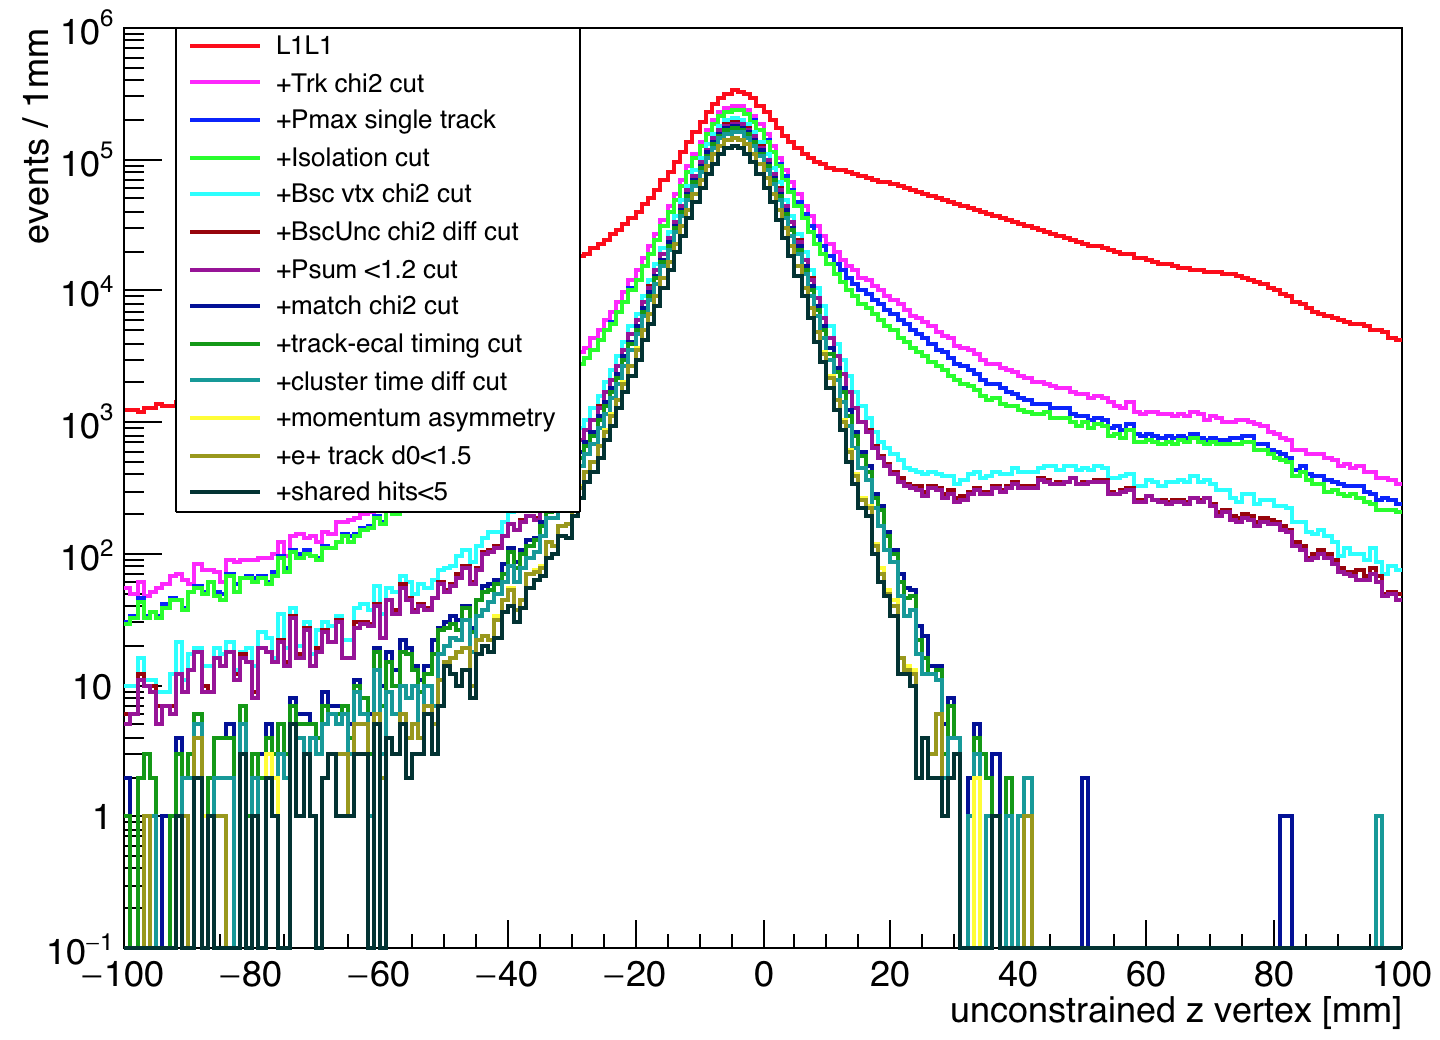
\includegraphics[width=0.8\textwidth]{plots/L1L1_zvtx.png}
  \caption{Cut effects on the z vertex distribution for all masses in the L1L1 0.5~mm dataset.}
  \label{fig:l1l1_vtx}
\end{figure} 

The ratio of the final events selected after applying all cuts to the original events selected after initial cuts is shown in Figure~\ref{fig:l1l1_vtxR}.

\begin{figure}[H]
  \centering
      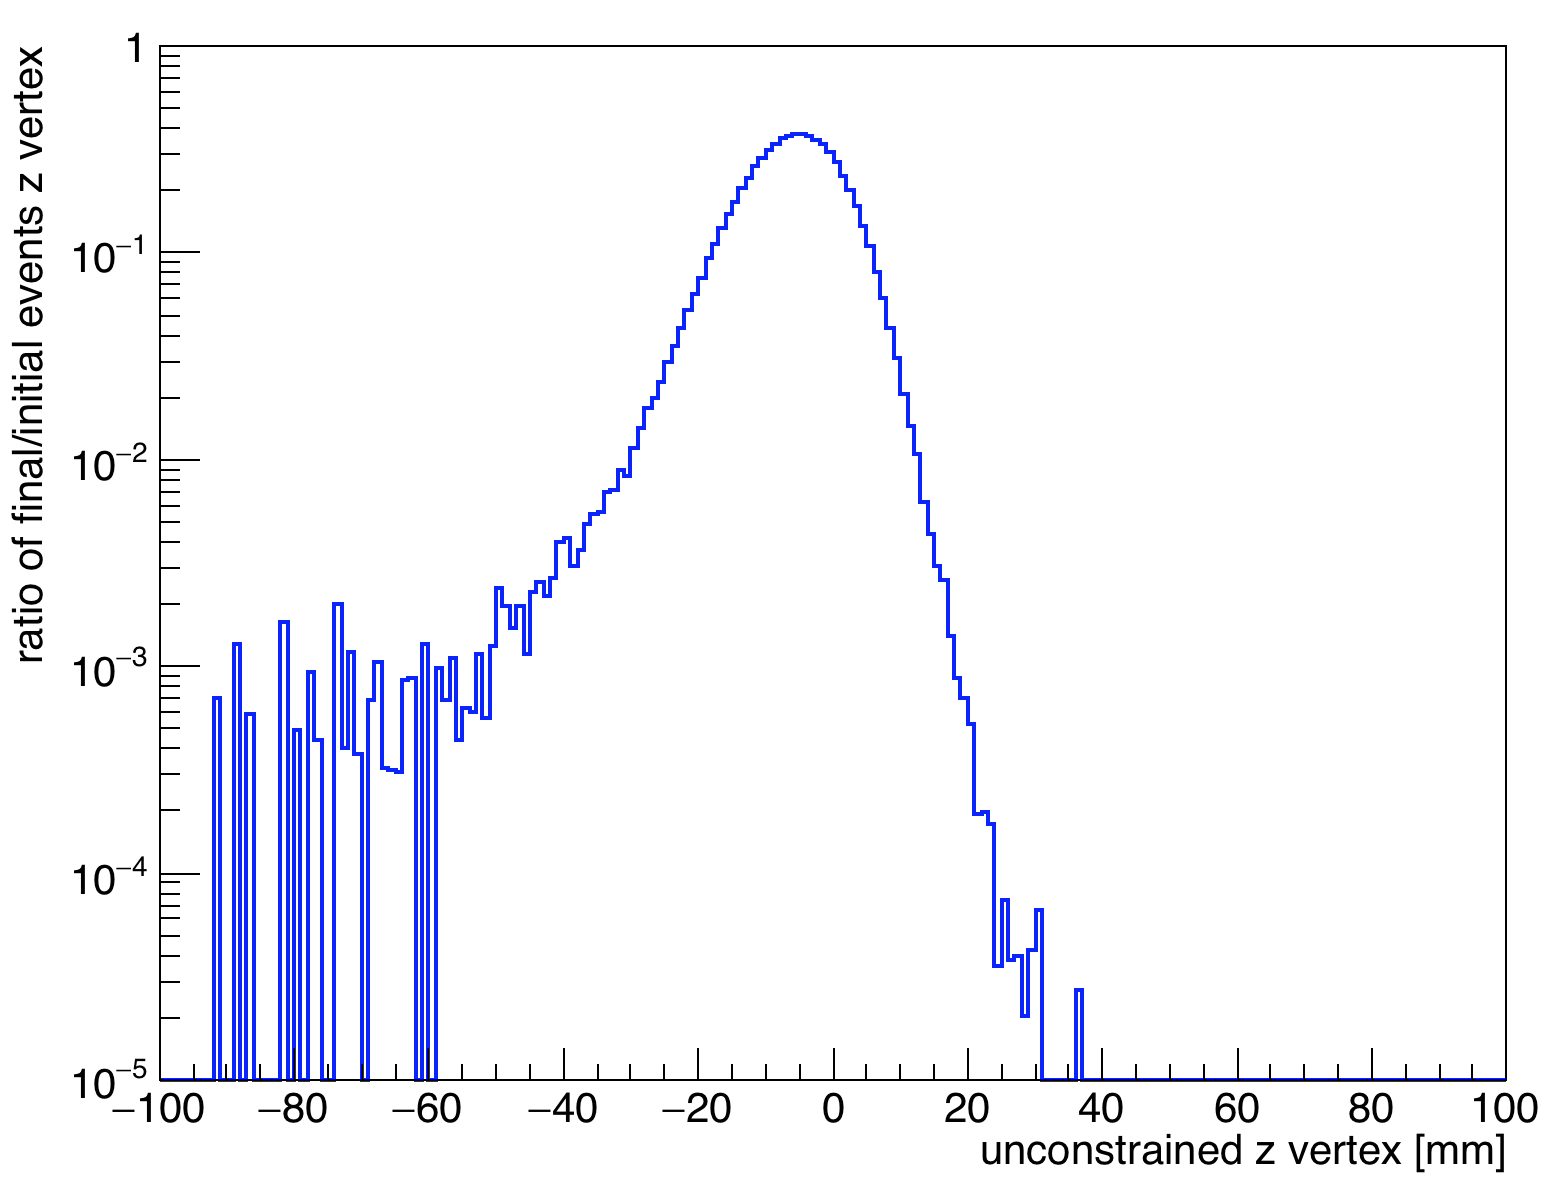
\includegraphics[width=0.8\textwidth]{plots/ratio_zvtx_cuts.png}
  \caption{The ratio of the z vertex distribution in the final event selection to those events in the initial event selection in the L1L1 0.5~mm dataset.}
  \label{fig:l1l1_vtxR}
\end{figure} 

The two cluster time difference can be used to study the effects of cuts on accidentals as well as the contamination of accidentals in the final sample. The evenly space 2~ns peaks as apparent in Figure~\ref{fig:l1l1_tdiff} are due to the intrinsic 499~MHz frequency at which electron beam bunches enter Hall B and interact with the HPS target. 

\begin{figure}[H]
  \centering
      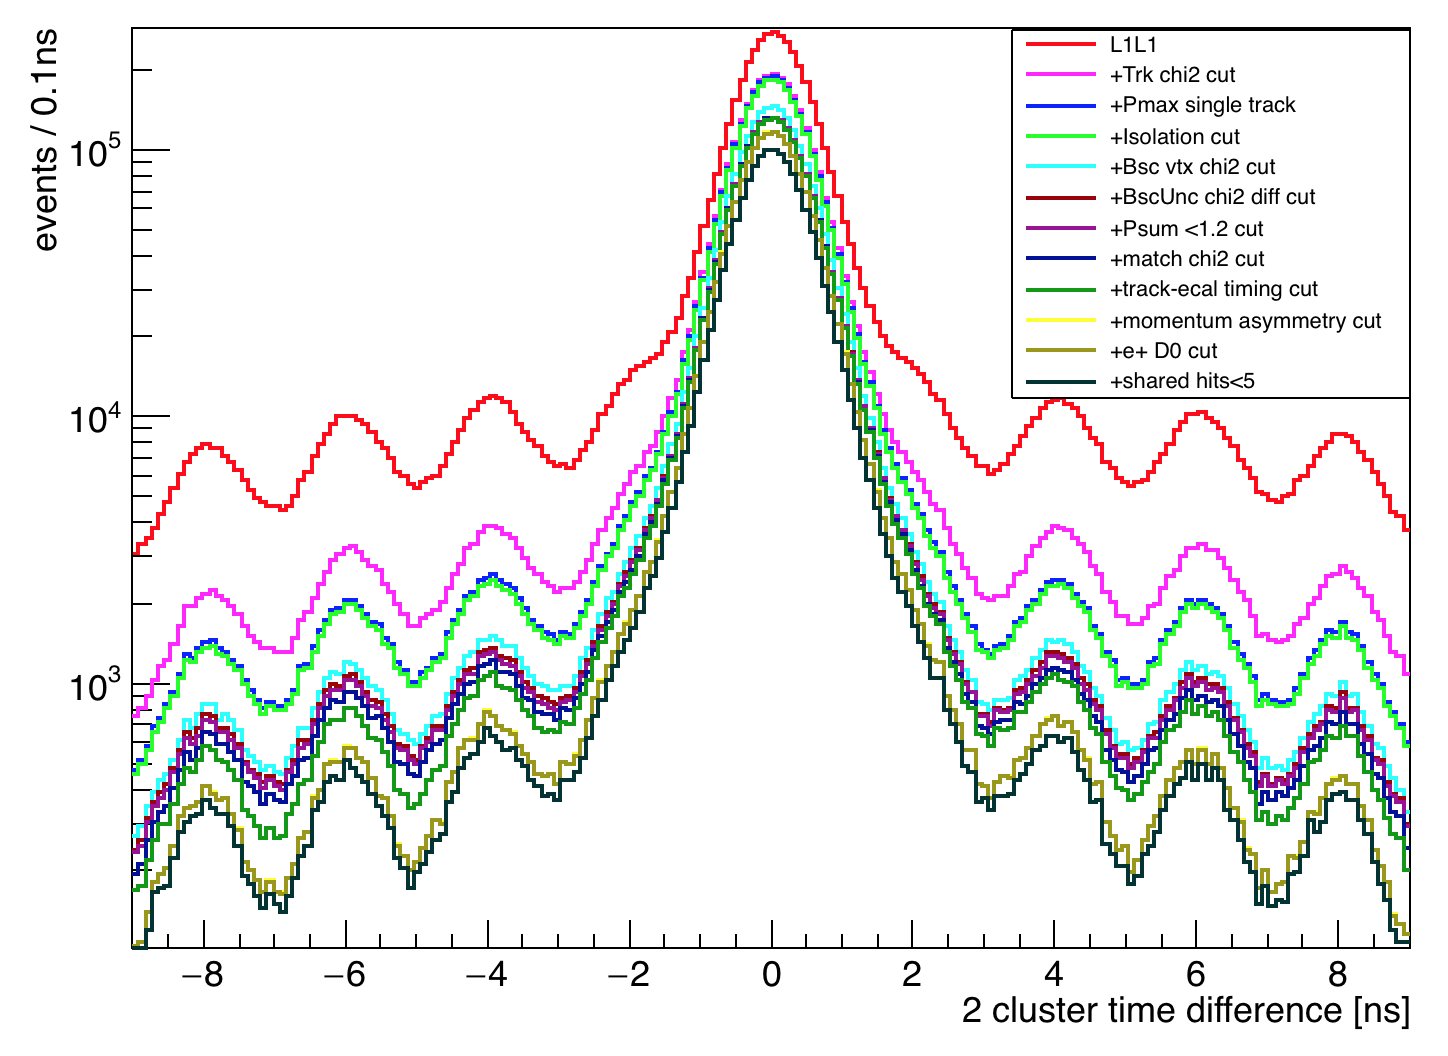
\includegraphics[width=0.8\textwidth]{plots/L1L1_tdiff.png}
  \caption{Cut effects on the two cluster time difference distribution for the L1L1 0.5~mm dataset.}
  \label{fig:l1l1_tdiff}
\end{figure} 

The effect of the cuts as shown in Figure~\ref{fig:l1l1_tdiff} on the final and initial distributions can be seen as a ratio in Figure~\ref{fig:l1l1_tdiffR}.

\begin{figure}[H]
  \centering
      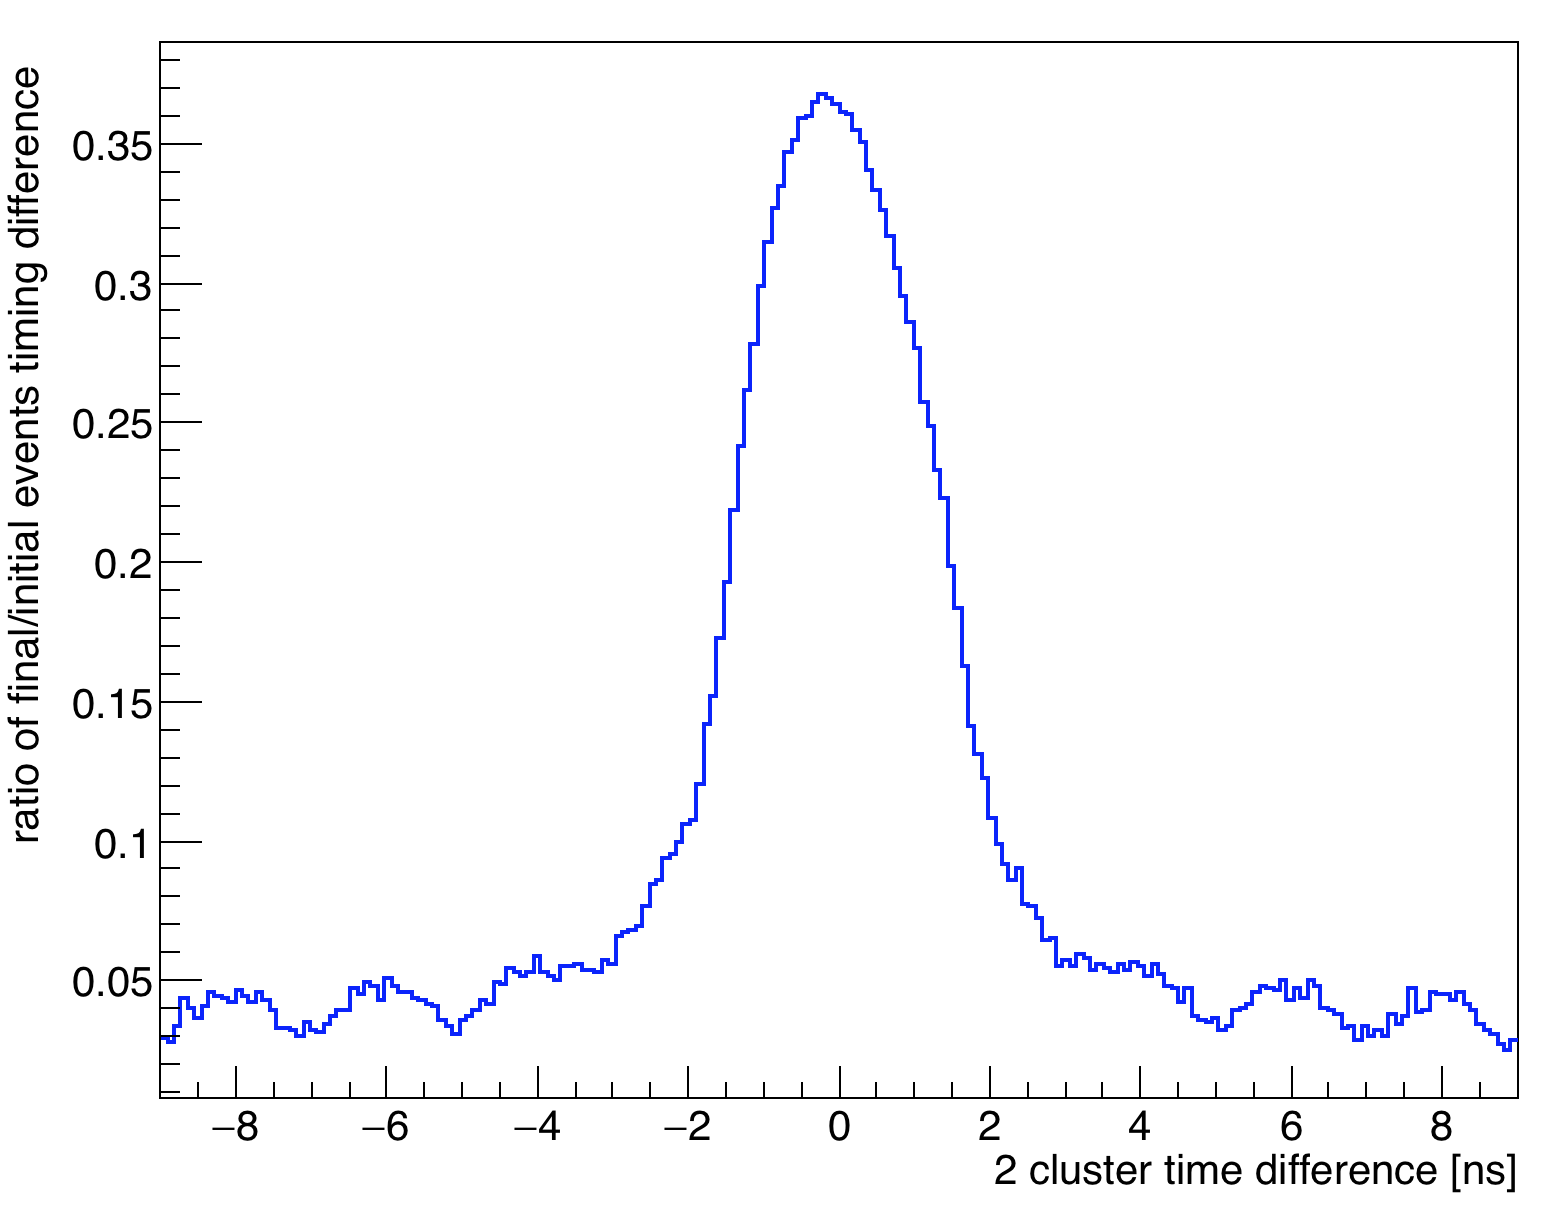
\includegraphics[width=0.8\textwidth]{plots/ratio_tdiff_cuts.png}
  \caption{The ratio of the two cluster time difference distribution in the final event selection (without the $\pm2$~ns cut) to those events in the initial event selection for the L1L1 0.5~mm dataset.}
  \label{fig:l1l1_tdiffR}
\end{figure}

After all cuts are applied, the accidental contamination is less than 1$\%$ in the $\pm$ 2~ns event selection (this cut is the only one not shown in Figure~\ref{fig:l1l1_tdiff}). Further studies to identify the production of high z vertices using accidentals is discussed later on in this section. The cut effects on the mass distribution for the vertex search can be seen in Figure~\ref{fig:l1l1_mass}. In particular, the track-cluster matching removes the low end tail of the mass distribution which is consistent with the geometric acceptance of the experimental setup.

\begin{figure}[H]
  \centering
      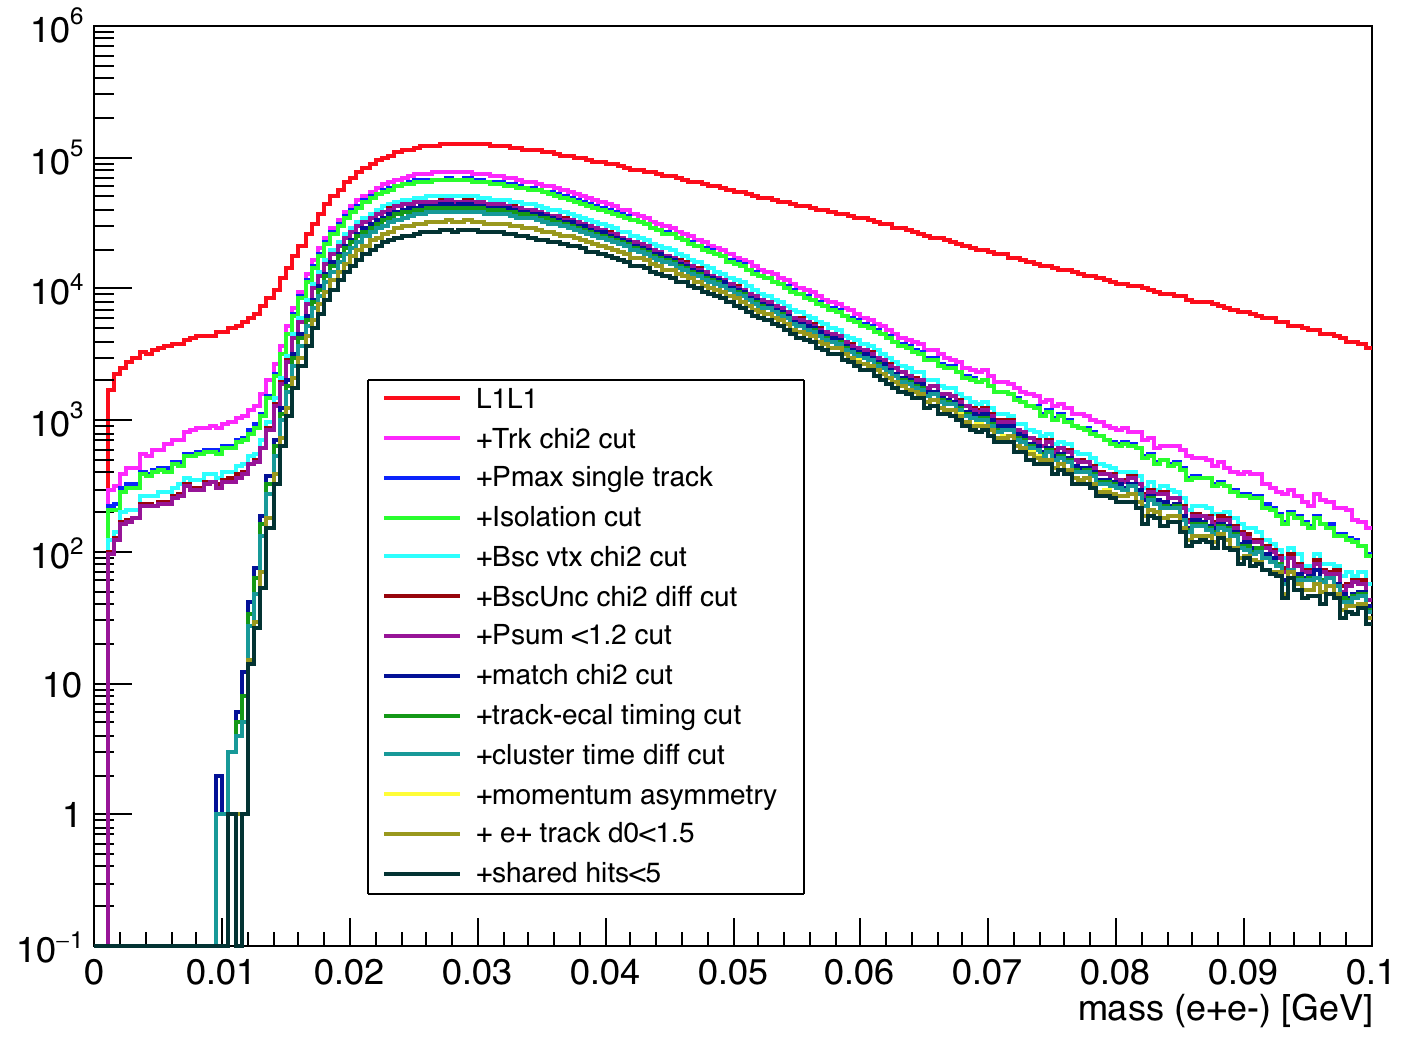
\includegraphics[width=0.8\textwidth]{plots/mass_L1L1_cuts.png}
  \caption{Cut effects on the mass distribution for the L1L1 0.5~mm dataset.}
  \label{fig:l1l1_mass}
\end{figure} 

An overview of the significant cuts will be discussed here. Any cut that is different from the L1L1 dataset will be discussed separately in the section with the relevant dataset. 

\indent The initial selection for the dataset requires that both tracks have hits in Layer 1 of the SVT and Layer 2. Previously, the requirement of Layer 2 was not used, but as the rates are highest in Layer 1 of the SVT, the extrapolation from Layer 3 to Layer 1 is critical in order to correctly measure the vertex of the track. Additionally, the inefficiency in measuring a hit in Layer 2 is approximately 2$\%$ of the time (and is different for electrons and positrons). Included in the initial event selection is also the radiative cut at 80$\%$ of the beam energy. After these initial cuts, we apply the track selection cuts. To ensure general track quality, the track $\chi^2$ is used as shown in Figure~\ref{fig:trkChi2}.

\begin{figure}[H]
  \centering
      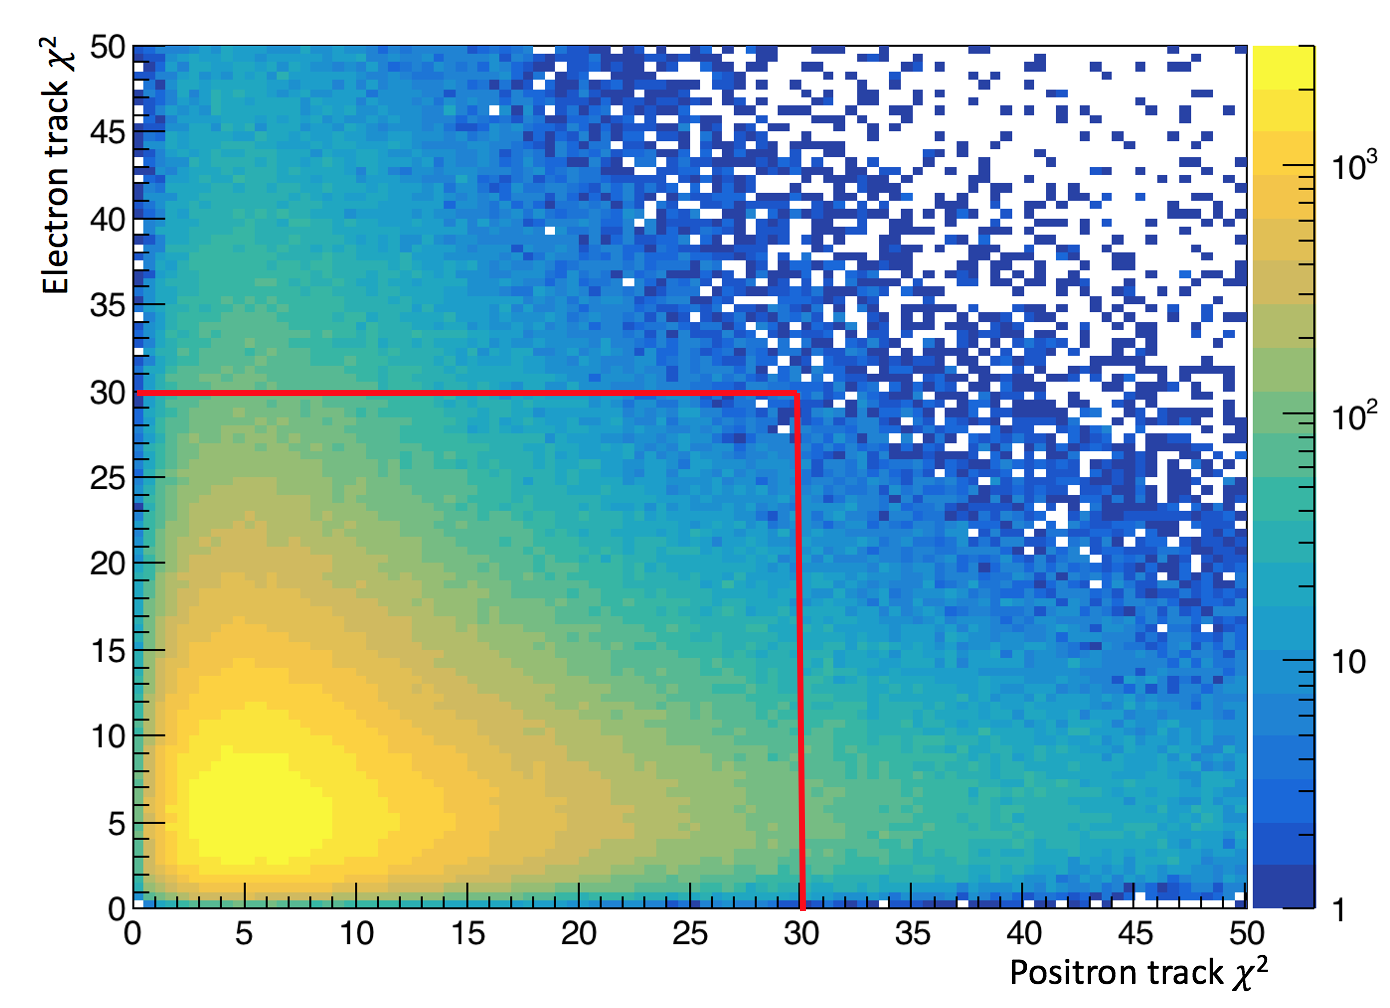
\includegraphics[width=0.8\textwidth]{plots/trkChi2.png}
  \caption{The electron and positron track $\chi^2$ are shown with the cut indicated by the red line. This cut is an initial track selection quality cut and uses no vertex or timing information.}
  \label{fig:trkChi2}
\end{figure} 

After choosing tracks based on their individual fit qualities, we remove electron tracks that have greater than 75$\%$ of the beam energy. This cut is made to ensure that we are not choosing elastically-scattered (beam energy) electrons and corresponds also to the general maximum value we can expect for an electron track in trident events. A comparison between the data and Monte Carlo is shown in Figure~\ref{fig:emTrkPmax}.

\begin{figure}[H]
  \centering
      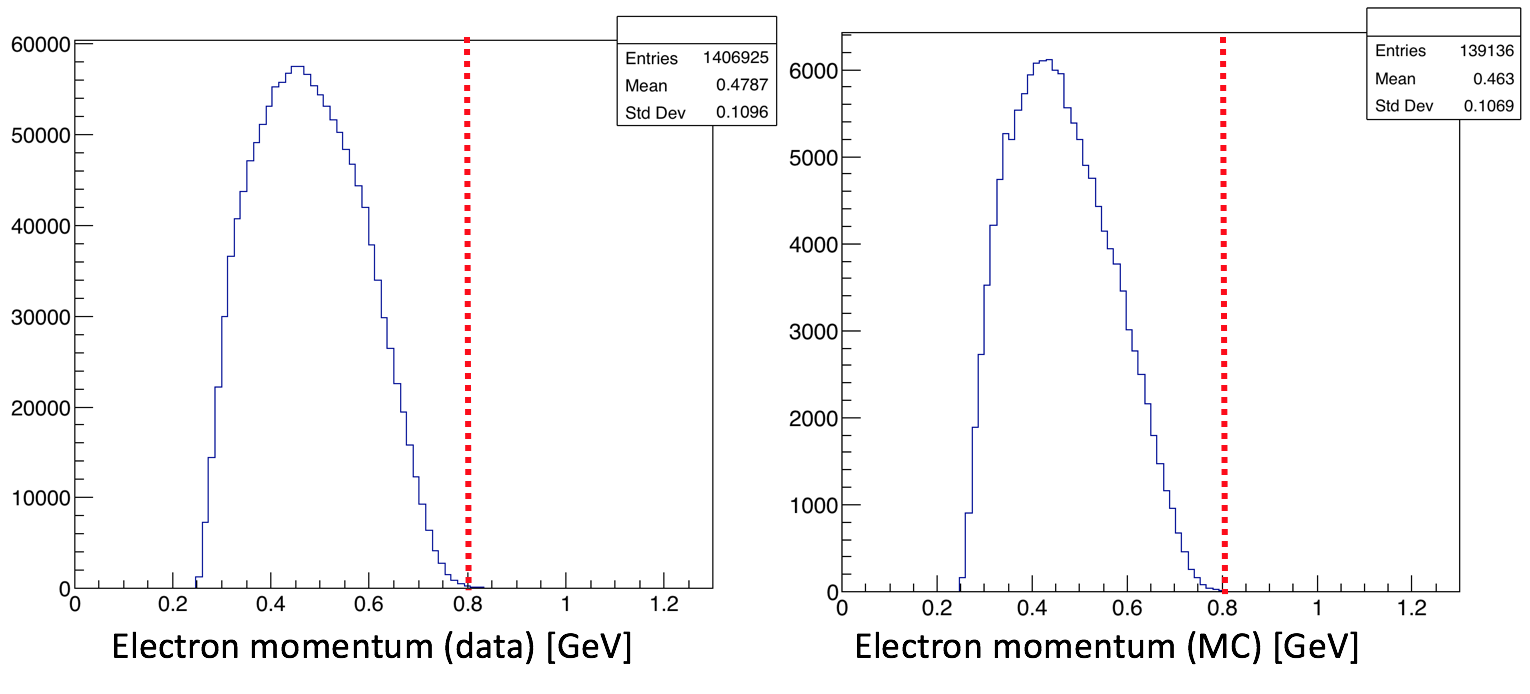
\includegraphics[width=0.8\textwidth]{plots/emTrkPmax.png}
  \caption{The maximum momentum of the electron track as shown in data (prior to cutting) and Monte Carlo. Events with higher electron energies are attributable to other types of backgrounds in the data such as elastics and wide angle bremsstrahlung and not the trident background.}
  \label{fig:emTrkPmax}
\end{figure} 

The next cut applied is the isolation cut. The isolation value for the electron and the positron in the L1L1 dataset is the distance to the next closest hit away from the beamline in Layer 1 relative to the electron and positron hit used in the track. This cut compares the isolation value (parameter $\delta$) to the track projected value in y at the target position (also known as the track $z0$ parameter). If the projected isolation to the target is larger than the $z0$ parameter at the target, then we assume that the better hit was already chosen for the track. A picture of the variables used in this cut is shown in Figure~\ref{fig:isoPic}.

\begin{figure}[H]
  \centering
      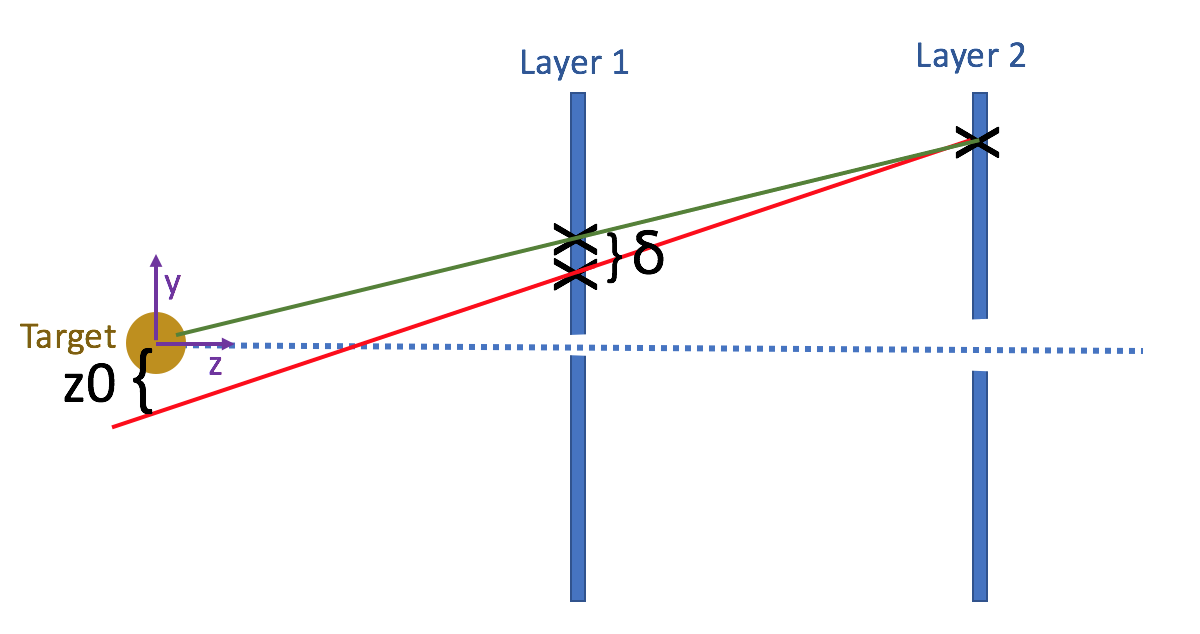
\includegraphics[width=0.8\textwidth]{plots/isolationPic.png}
  \caption{The distance between the closest hit away from the beam in Layer 1 is compared to its projection at the target the track impact parameter, $z0$ at the target. }
  \label{fig:isoPic}
\end{figure}

The cut shown is described numerically in Equation~\eqref{eq:isolationl1}.

\begin{equation}
\label{eq:isolationl1}
2\delta+z0\times\textbf{sign($PY$)}>0
\end{equation}
 
Because the distance from Layer 2 to the target is twice the distance between Layer 1 and the target, we compare the isolation times a factor of 2 to the $z0$ parameter in order to compare the projection to the target. The $z0$ parameter is opposite in sign as compared to the y-component of the track momentum because we only consider downstream vertices. 


\indent In identifying downstream vertices, we use the unconstrained vertex collection to optimize our search for detached vertices. For each vertexed $e+e-$ pair, we can see how the vertex is changed when different additional constraints are applied to the vertex. The unconstrained vertex collection only looks at the distance of closest approach between the two tracks. The target constrained vertex collection is optimized for a bump hunt analysis and requires that the vertex of the $e+e-$ pairs occurs at the target. The beamspot constrained vertex collection requires that the momentum of the vertexed pairs projects back to the beamspot location at the target and considers the distance of closest approach between the two tracks. 

The beamspot constrained vertex $\chi^2$, can give us information about how well the vertex momentum points back to the beamspot location at the target. The beamspot constraint is particularly useful in identifying events where a track has scattered significantly because the the projected momentum misses the beamspot location at the target. Real signal will always project back to the beamspot. The effect of the beamspot constraint cut on the vertex  $\chi^2$ distribution alone can be seen in Figure~\ref{fig:bsccut}.

\begin{figure}[H]
  \centering
      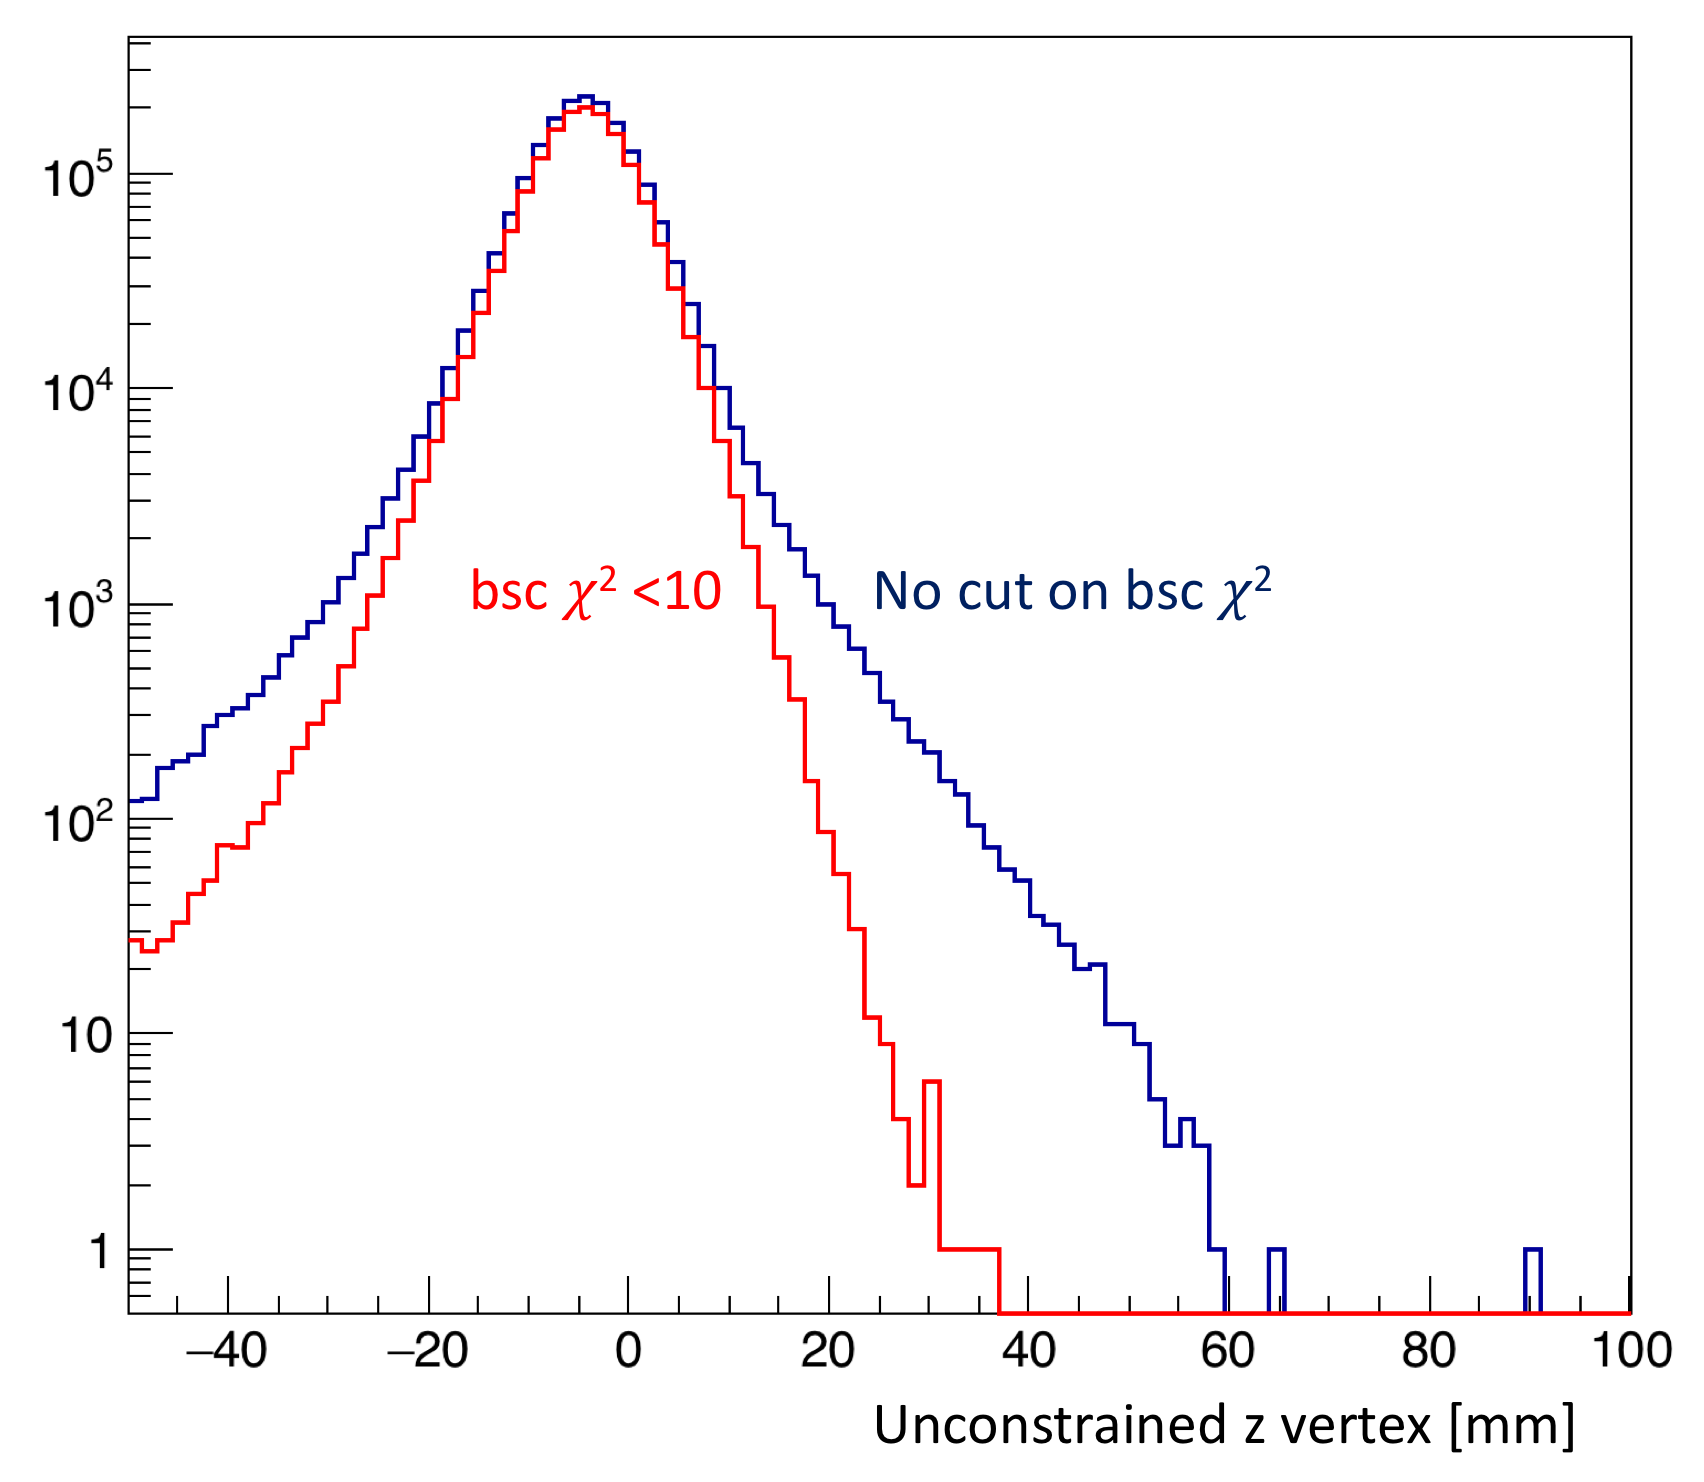
\includegraphics[width=0.6\textwidth]{plots/bscCut.png}
  \caption{The effect of a cut on the beamspot constrained $\chi^2$ on the vertex distribution for all masses. While this plot is shown for all masses, the effects of the cut on the tails of the distribution can still be seen. The cut removes events where tracks did not pass close to eachother in space to generate a vertex and/or the vertex does not point back to the beam position at the target.}
  \label{fig:bsccut}
\end{figure} 

The difference between the beamspot constrained and unconstrained $chi^2$ can also be used to exclusively identify how well a vertex points back to the target. The effect of this cut can be seen in Figure~\ref{fig:bmucut}.

\begin{figure}[H]
  \centering
      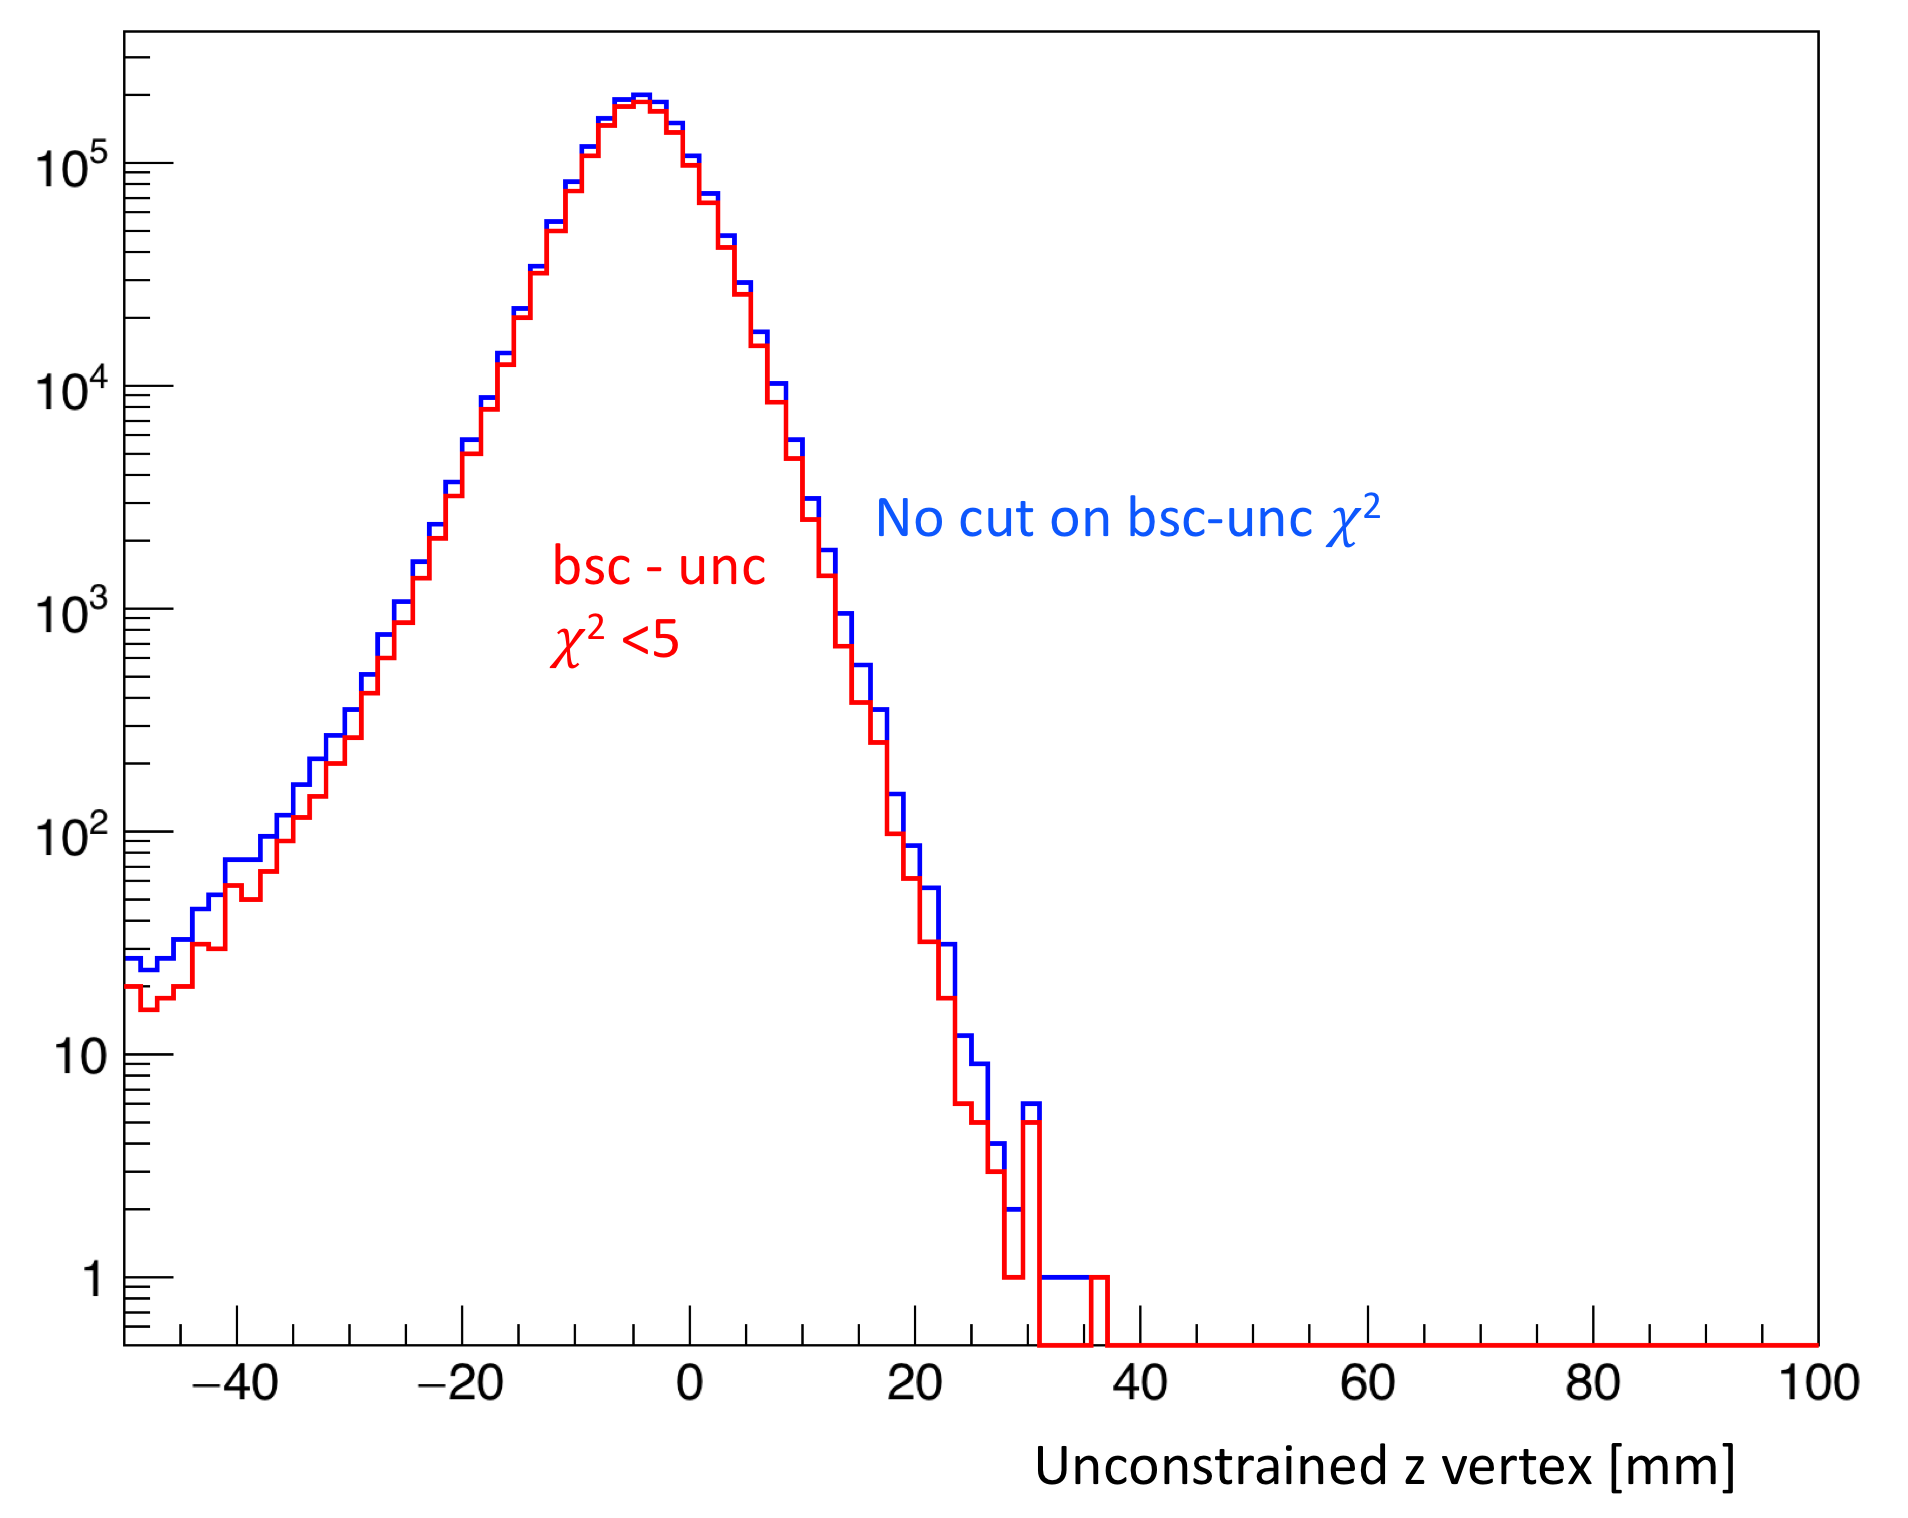
\includegraphics[width=0.6\textwidth]{plots/bmuchi2.png}
  \caption{The effect of a cut on the difference between the beamspot and unconstrained constrained $\chi^2$ on the vertex distribution for all masses. The effects of the cut on the downstream tails of the distribution tells us how well a vertexed pair of tracks points back to the beamspot position at the target.}
  \label{fig:bmucut}
\end{figure} 

The next cut is the maximum momentum of the $e+e-$ pair. This cut removes very few events but is still necessary to ensure that we are not including events that are not correlated. After having established the quality of the tracks and vertex using the SVT information only, the tracks are projected to their positions at the Ecal and the quality of the matching of the track and Ecal cluster is described as a function of the track momentum and position at the Ecal. This parameter is a function of the number of $\sigma$ from distributions studied used 2015 data. The matching parameter and relevant cut value are shown in Figure~\ref{fig:matchcut}. 

\begin{figure}[H]
  \centering
      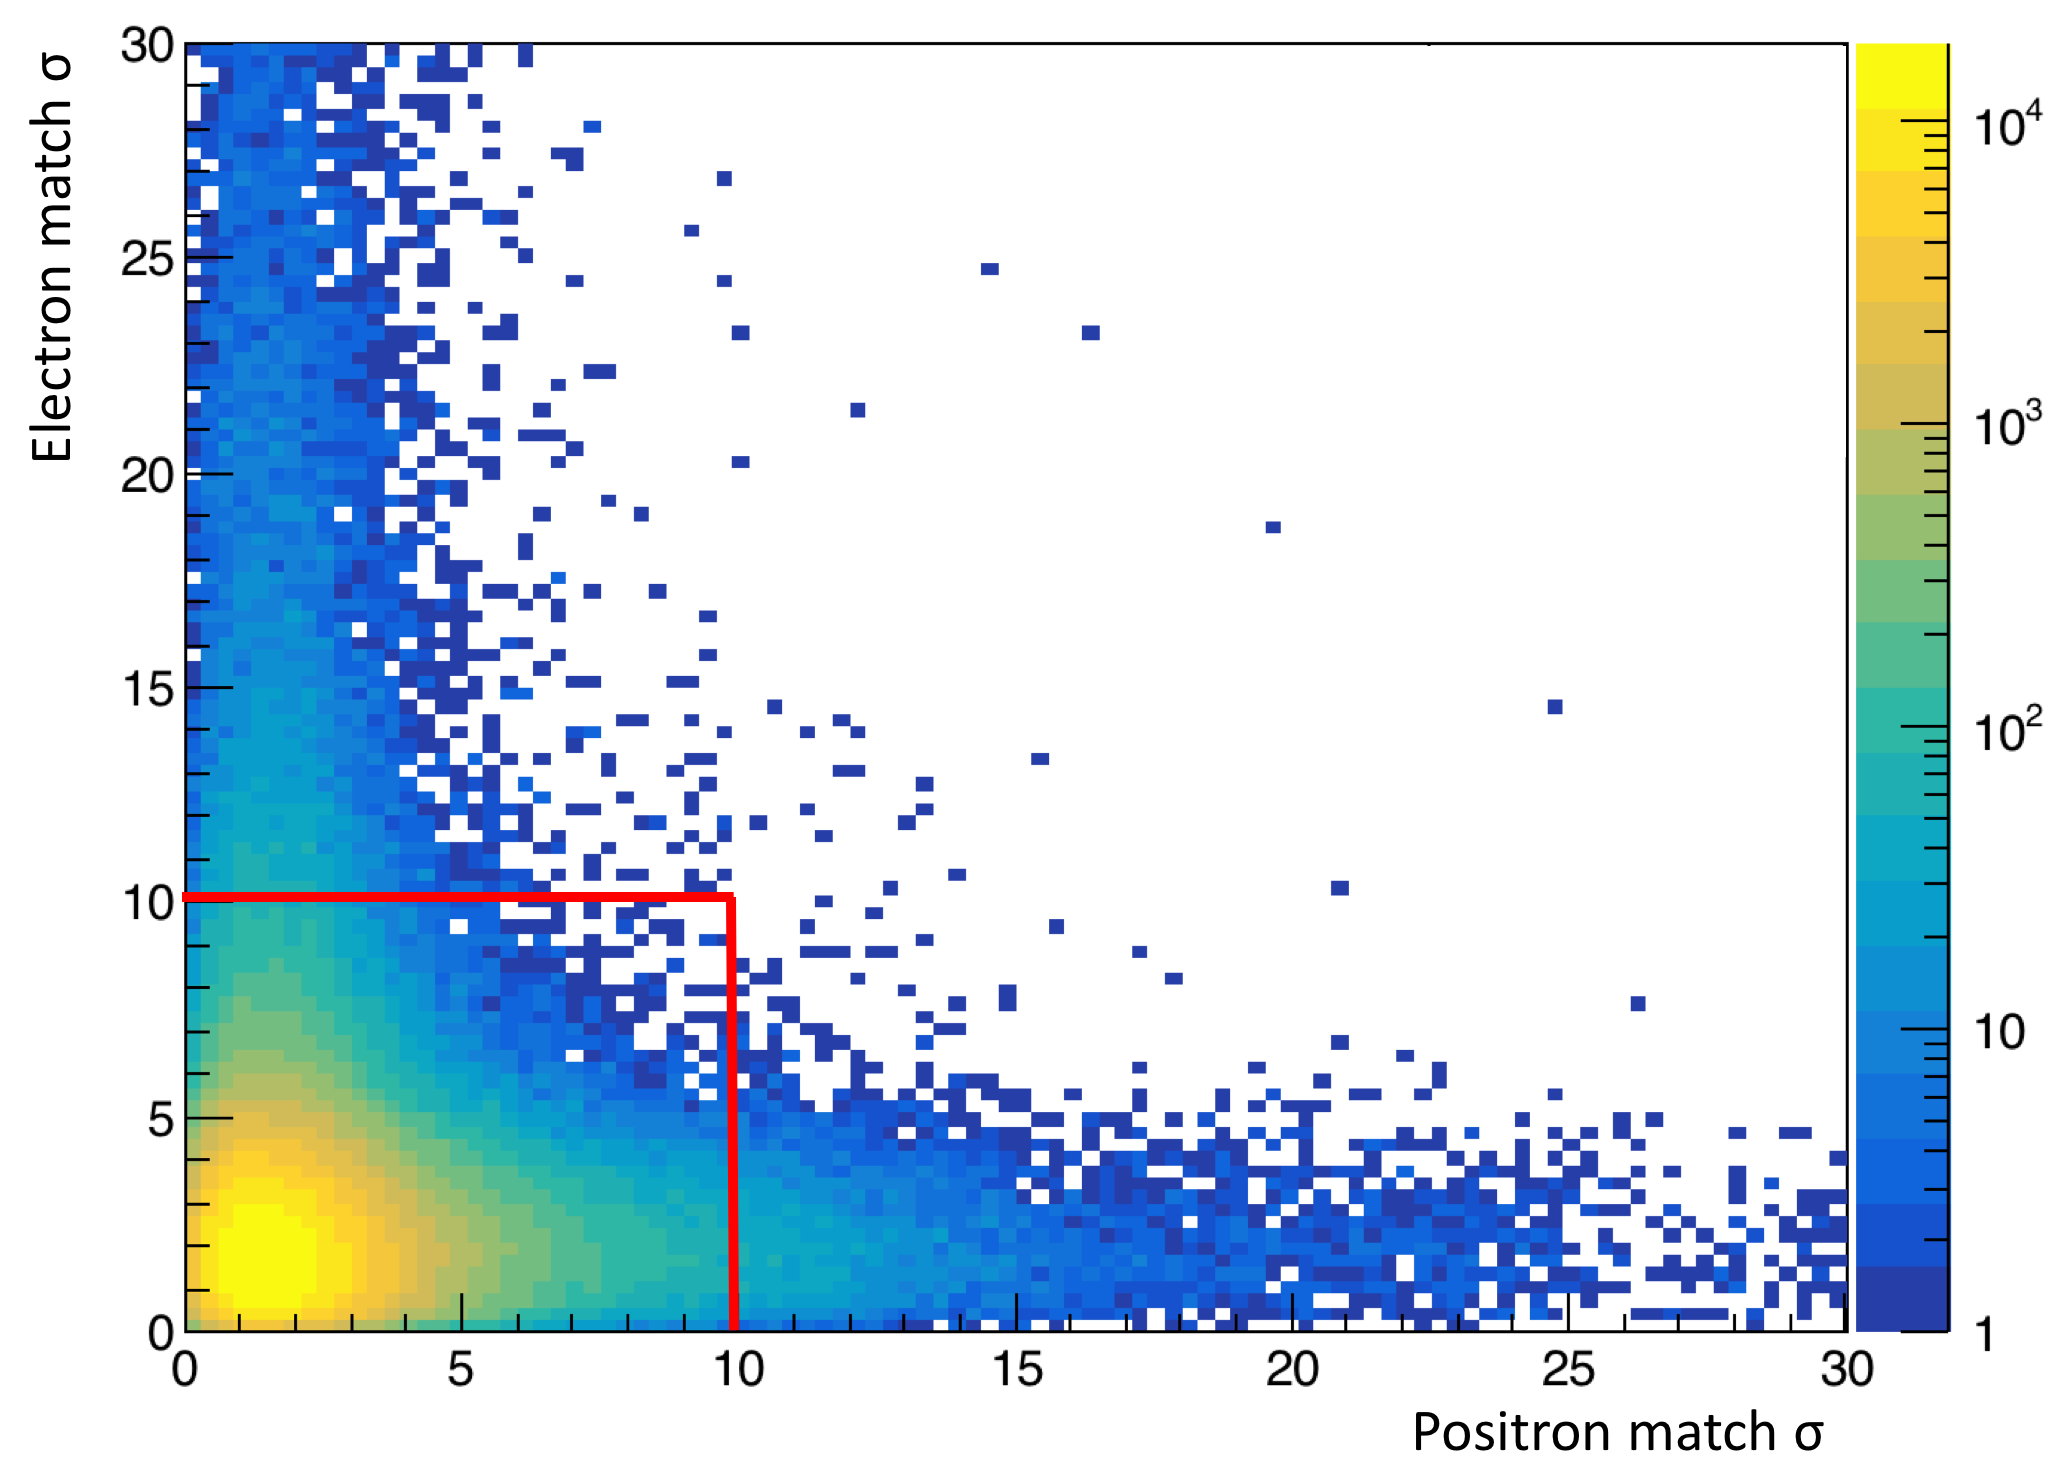
\includegraphics[width=0.8\textwidth]{plots/matchcut.png}
  \caption{The matching parameter for both electrons and positrons is shown. The maximum is set to 30$\sigma$, and the cut is set to 10$\sigma$ for each particle.}
  \label{fig:matchcut}
\end{figure} 

The matching cut most significantly removes the small angle/low mass background events that we saw in Figure~\ref{fig:l1l1_mass}. The timing difference between the tracks and Ecal clusters removes some out of time events, but the timing resolution on the clusters is more precise than the track time and a cut on the two cluster time difference is critical for removing accidentals. The cut can be seen in Figure~\ref{fig:cltdiff}.

\begin{figure}[H]
  \centering
      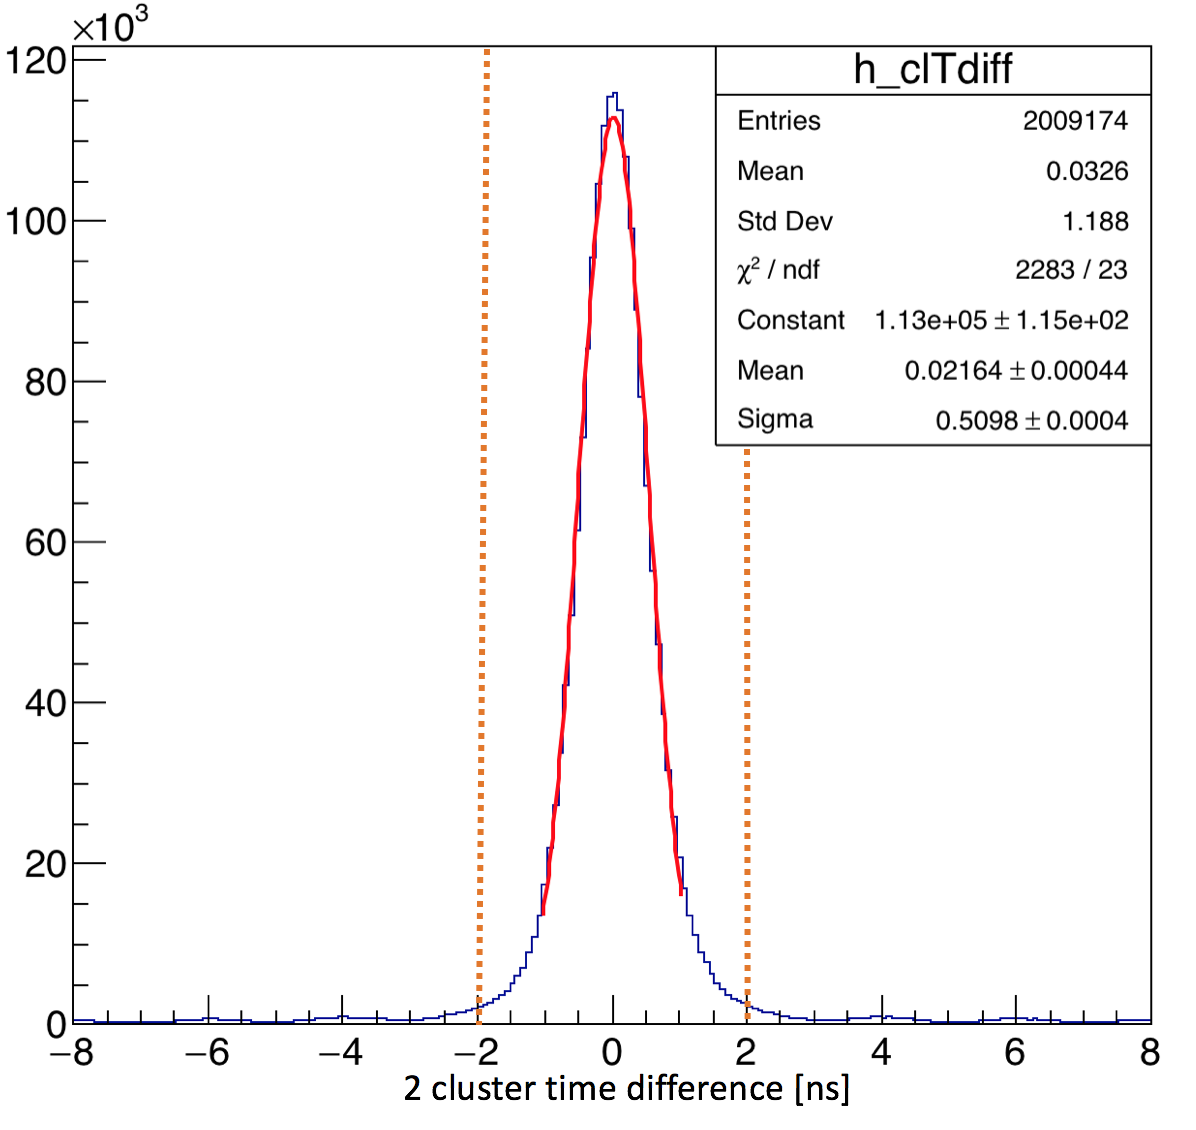
\includegraphics[width=0.6\textwidth]{plots/cltdiff.png}
  \caption{The two cluster timing difference is shown with a fit to the Gaussian central part of the distribution. Additional smaller peaks can be seen in intervals of 2~ns in the tails of the distribution. The timing cut can remove these events where overlapping beam buckets generate out of time vertices.}
  \label{fig:cltdiff}
\end{figure} 

Additional cuts aimed to remove the contaminating wide angle breamsstrahlung background events include a cut on the momentum asymmetry of the two tracks and the positron $D0$, or $DOCA$ (distance of closest approach to the target in the x-z plane), are used. The $e+e-$ pairs produced in radiative trident processes from heavy photon decays are closely symmetric in momentum. The momentum asymmetry is defined as the momentum difference of the two particles divided by the momentum sum. The electron in wide-angle bremsstrahlung typically carries a significantly higher portion of the beam energy when compared to the positron that is produced from the pair production of the lower energy photon. The effects of the momentum asymmetry cut on the vertex distribution are shown in Figure~\ref{fig:pasycut}.

\begin{figure}[H]
  \centering
      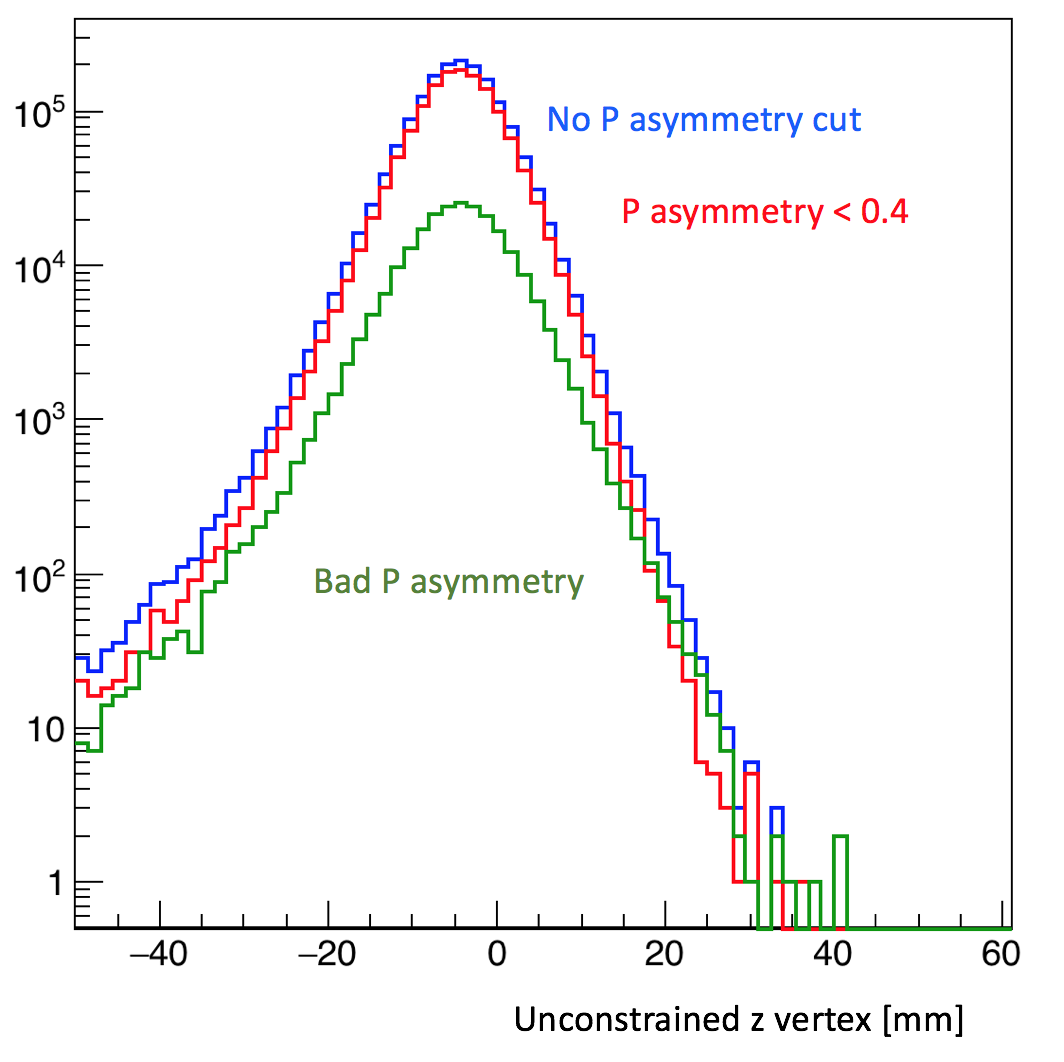
\includegraphics[width=0.6\textwidth]{plots/pasycut.png}
  \caption{The effect of the momentum asymmetry cut on the tails of the vertex distribution can be seen in the red an green curves.}
  \label{fig:pasycut}
\end{figure} 

The momentum asymmetry cut can effectively reduce contamination from wide-angle bremsstrahlung in the final event sample. In wide-angle bremsstrahlung, the scattered electron and the positron from pair conversion are detected. When a positron is produced downstream of the target in this process, the projected $DOCA$ of the resultant track to the target will be positive due to the curvature of the positron track in the magnetic field from starting downstream. The cut on the $DOCA$ and its effect on the vertex distribution can be seen in Figure~\ref{fig:docacut}. 

\begin{figure}[H]
  \centering
      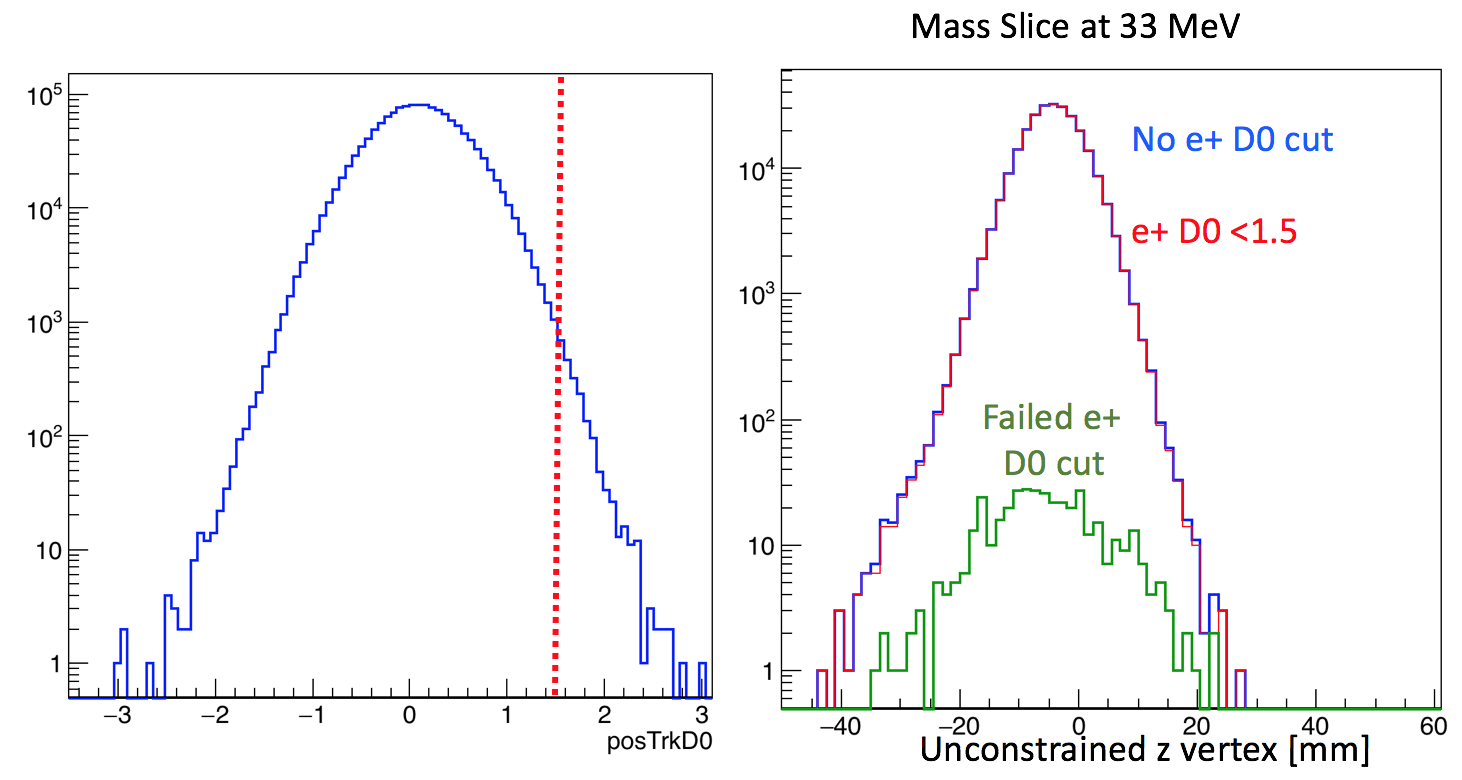
\includegraphics[width=0.8\textwidth]{plots/docacut.png}
  \caption{Positrons that are produced from the photon in wide-angle bremsstrahlung events will have a distance of closest approach that will curve widely at the target location, yielding a largely positive value.}
  \label{fig:docacut}
\end{figure} 

The final cut on tracks was derived after studies of the high z background events showed a higher probability of one or both of the tracks sharing five hits with another track in the event. In these cases, the track with the best $\chi^2$ track fit is selected, but the momentum difference with the other track with which it shares five hits is quite small. The momentum difference of the track with the other tracks that share hits is shown versus the number of hits shared between the tracks in Figure~\ref{fig:trkshare}.

\begin{figure}[H]
  \centering
      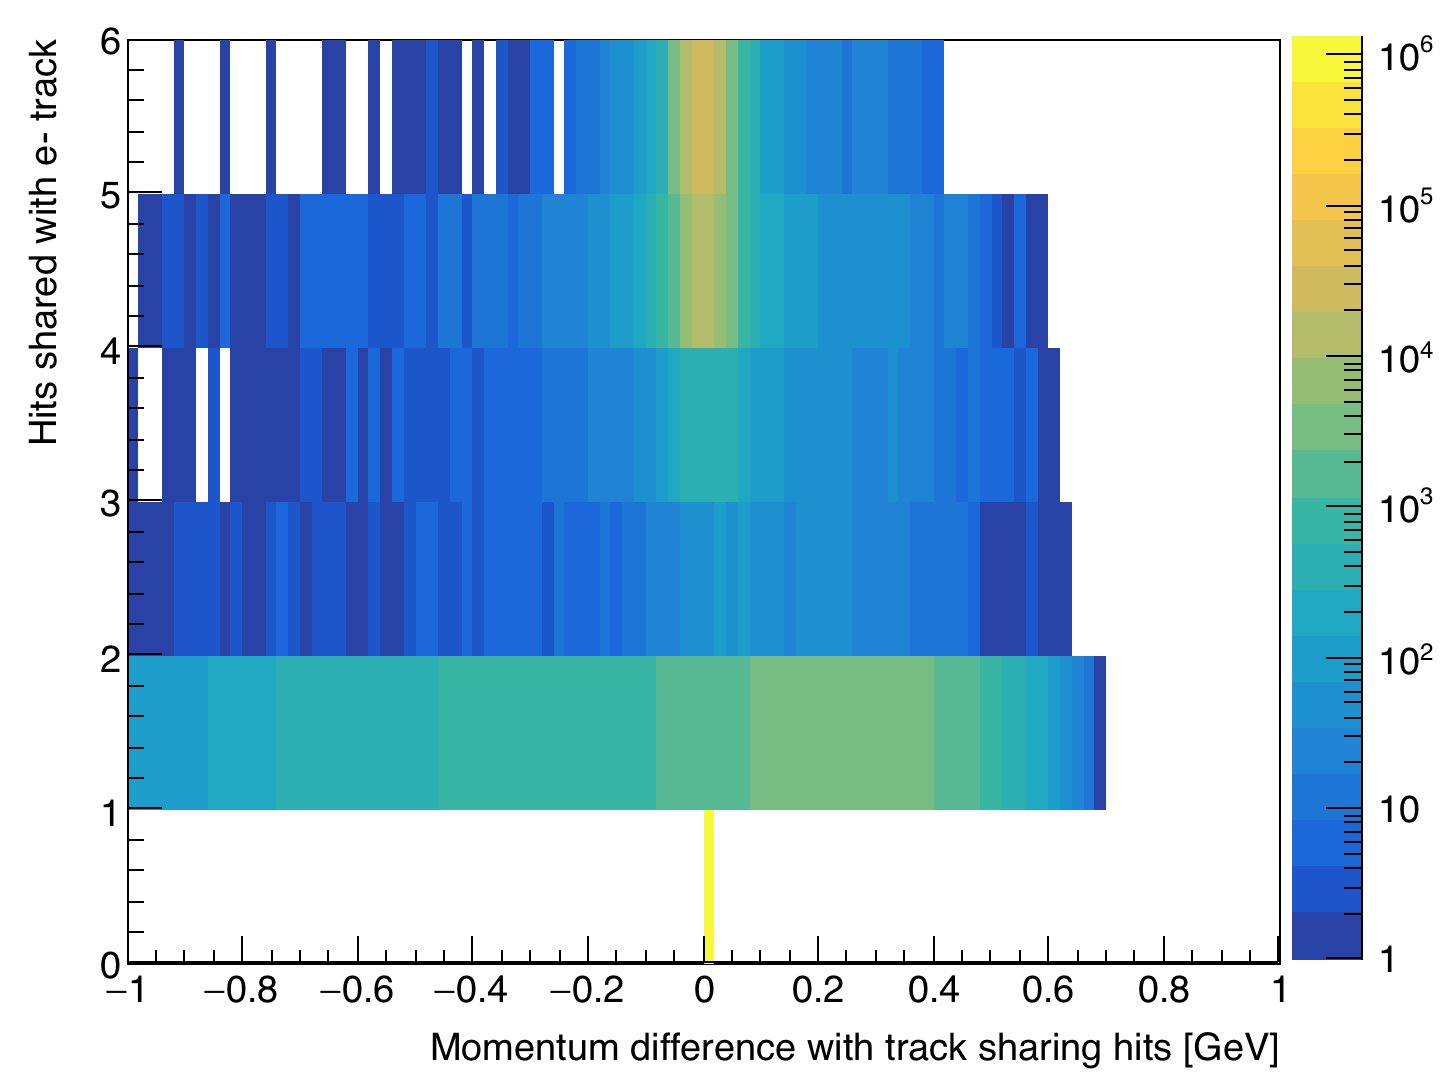
\includegraphics[width=0.8\textwidth]{plots/TrkShareHits.png}
  \caption{This plot shows that many of the tracks sharing 4 and 5 hits with the initial track selected in the event have nearly the same momentum.}
  \label{fig:trkshare}
\end{figure} 

By removing tracks that only have a one hit difference with other tracks, the high z background in the unblinded sample is reduced.   


\subsubsection{Vertex reconstruction efficiency, $\epsilon_{vtx}$}

The integral as described in Equation~\eqref{eq:signal} contains an $\epsilon_{vtx}$ parameter that varies as a function of both mass and vertex position z. Using A' Monte Carlo, the $\epsilon_{vtx}$ can be calculated and the efficiency can be parameterized as a funtion of mass and $z$. At each mass, the ratio of the measured to generated heavy photon events is scaled such that for L1L1, the fitted ratio is 1 at that target position. The L1L2 and L2L2 datasets are scaled to ensure the same relative relationship between the three datasets. The efficiencies for a 35~MeV heavy photon are shown in Figure~\ref{fig:apEff}. 

\begin{figure}[H]
  \centering
      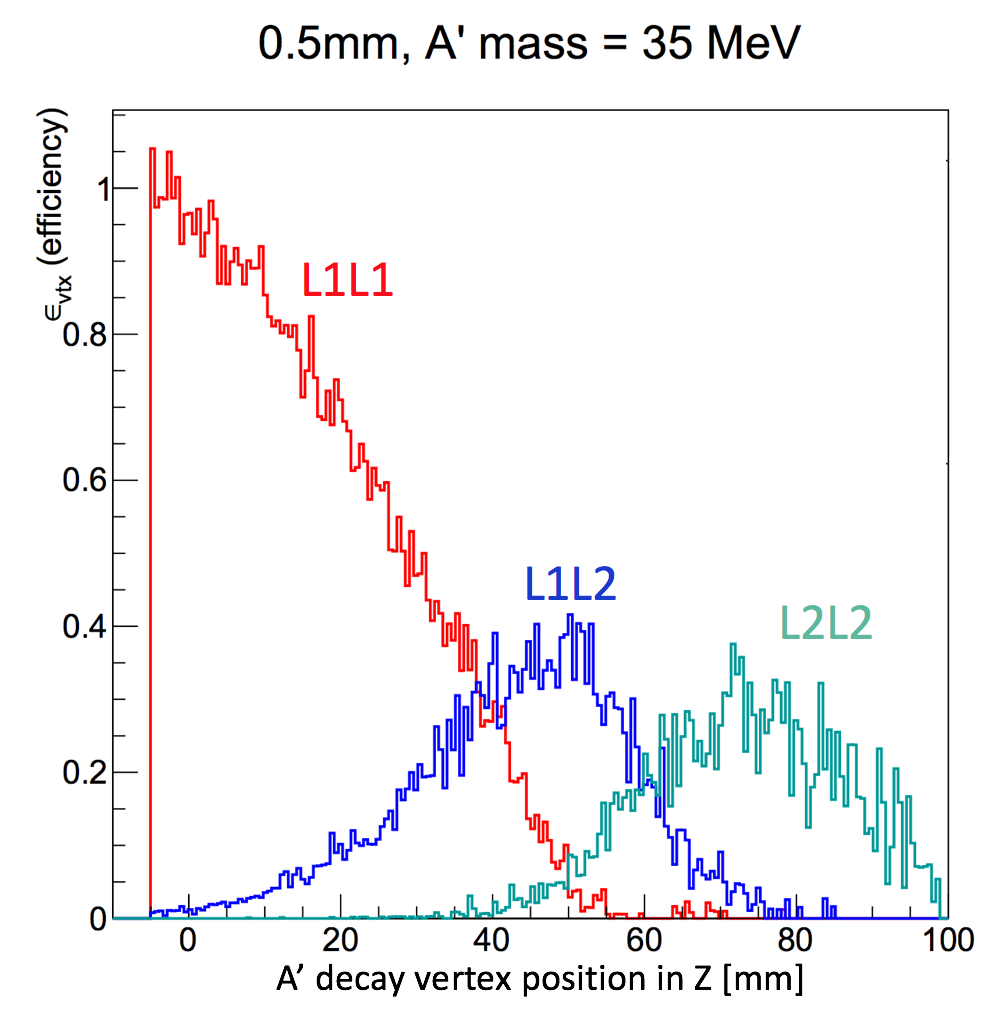
\includegraphics[width=0.8\textwidth]{plots/35MeV_apEff.png}
      \caption{35~MeV A' reconstruction efficiency versus the vertex position.}
        %The efficiencies for all masses can be seen in a file at\\ \href{url}{https://userweb.jlab.org/~hszumila/vertexNote/vertexEffFitsCombined.pdf}.}
  \label{fig:apEff}
\end{figure} 

As all datasets are mutually exclusive of eachother, one can see that the total reconstruction efficiency for all z vertex positions is the sum of the efficiencies for the individual datasets as shown in Figure~\ref{fig:apEff}. These efficiencies are then integrated from different zCut values to zMax (roughly set at the z position of Layer 1). The efficiency at each mass is for each dataset is fit as shown for a 30~MeV heavy photon in Figure~\ref{fig:effFitted}.

\begin{figure}[H]
  \centering
      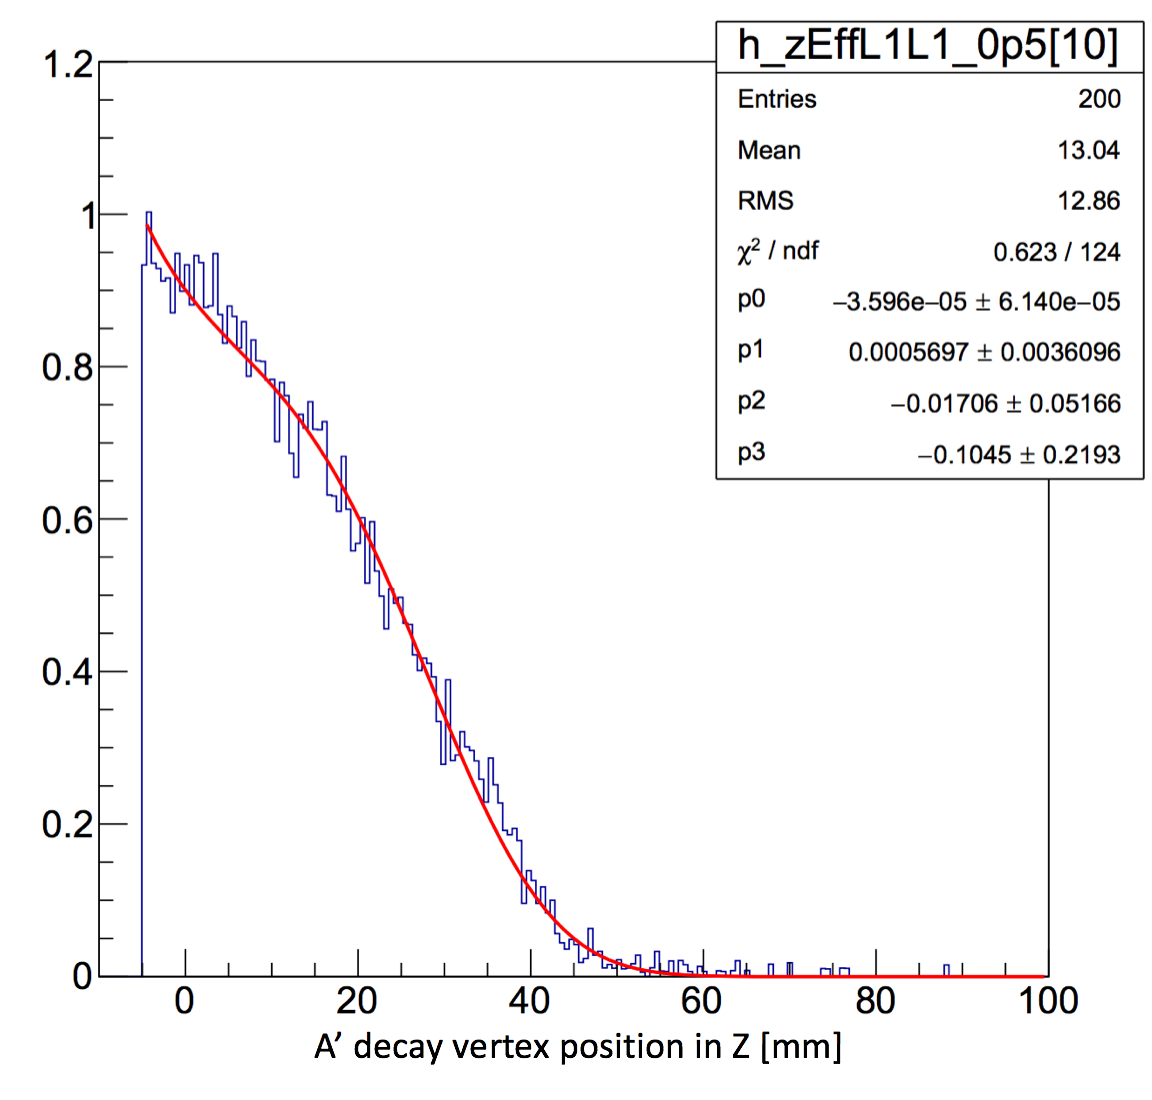
\includegraphics[width=0.8\textwidth]{plots/L1L1_eff_35MeV.png}
      \caption{Fit that describes the L1L1 efficiency for a 30~MeV heavy photon.}
        %All masses are saved to a file at\\
  %\href{url}{https://userweb.jlab.org/~hszumila/vertexNote/vertexEffFits.pdf}.}
  \label{fig:effFitted}
\end{figure} 

The parameters of the fits to all masses are then parameterized as a function of mass. Once these relations are derived, then we obtain a value for $\epsilon_{vtx}$ that can be used in the integration for calculating the expected A' signal yield. For L1L1, the vertex reconstruction efficiency can be described as shown in in Equation~\eqref{eq:epsVtxL1}.

\begin{equation}
\label{eq:epsVtxL1}
\epsilon_{vtx} = exp(p_0+p_1z+p_2z^2+p_3z^3) 
\end{equation}

The parameters in Equation~\eqref{eq:epsVtxL1} are functions of mass and are shown below:
\begin{eqnarray*}
\label{eq:parsEpsVtxL1}
p_0 & = & -0.2359+3.606m\\
p_1 & = & -0.03537+0.5395m \\
p_2 & = & -0.001201+0.1404m-2.614m^2+10.65m^3 \\
p_3 & = & -0.0002078+0.008753m-0.1396m^2+0.8077m^3\\
\end{eqnarray*}

The full integral value yields some fractional number that, when multiplied by the expected heavy photon yield from the cross section, tells us how many heavy photons we can expect to reconstruct in the given decay vertex region. For the L1L1 dataset, it is critical to set the zCut as low as possible in order to obtain the highest signal yield. In Figure~\ref{fig:integratedVal2D}, the value of the integral indicated by the color on the z-axis, is shown for $\epsilon^{2} = 5E-9$ as a function of mass and zCut. The zMax was set to 100~mm in this calculation. 

\begin{figure}[H]
  \centering
      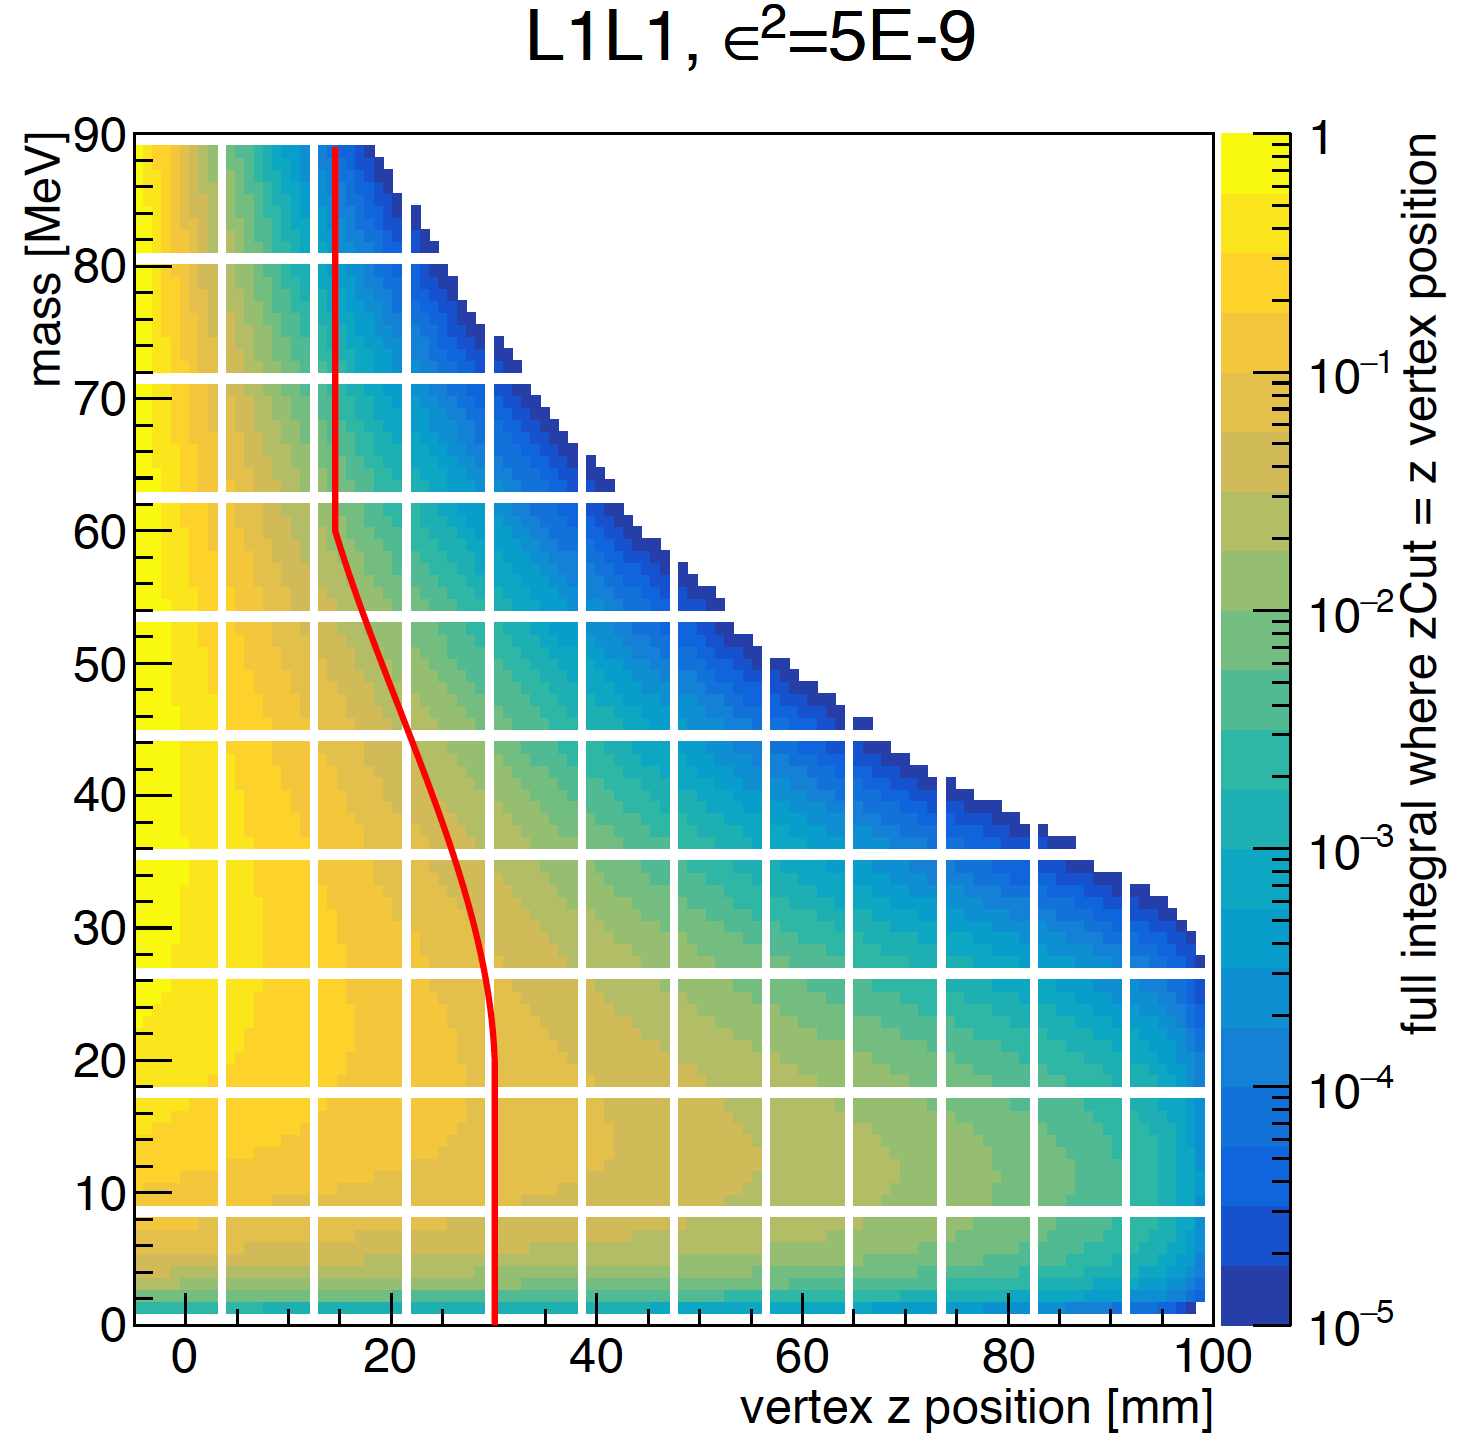
\includegraphics[width=0.8\textwidth]{plots/L1L1_eff_mz.png}
  \caption{The colored value is the value of the full integral from Equation~\eqref{eq:signal} for the L1L1 dataset using the zCut value on the x-axis. The red line indicates the zCut value derived in data for 0.5 background events. This zCut shown is for the 10$\%$ unblinded data.}
  \label{fig:integratedVal2D}
\end{figure} 

The red line shown in Figure~\ref{fig:integratedVal2D} indicates the zCut projection for the 10$\%$ unblinded L1L1 dataset. In Figure~\ref{fig:integratedVal1D}, the integral from this zCut to 100~mm is shown as a function of mass for various couplings. 

\begin{figure}[H]
  \centering
     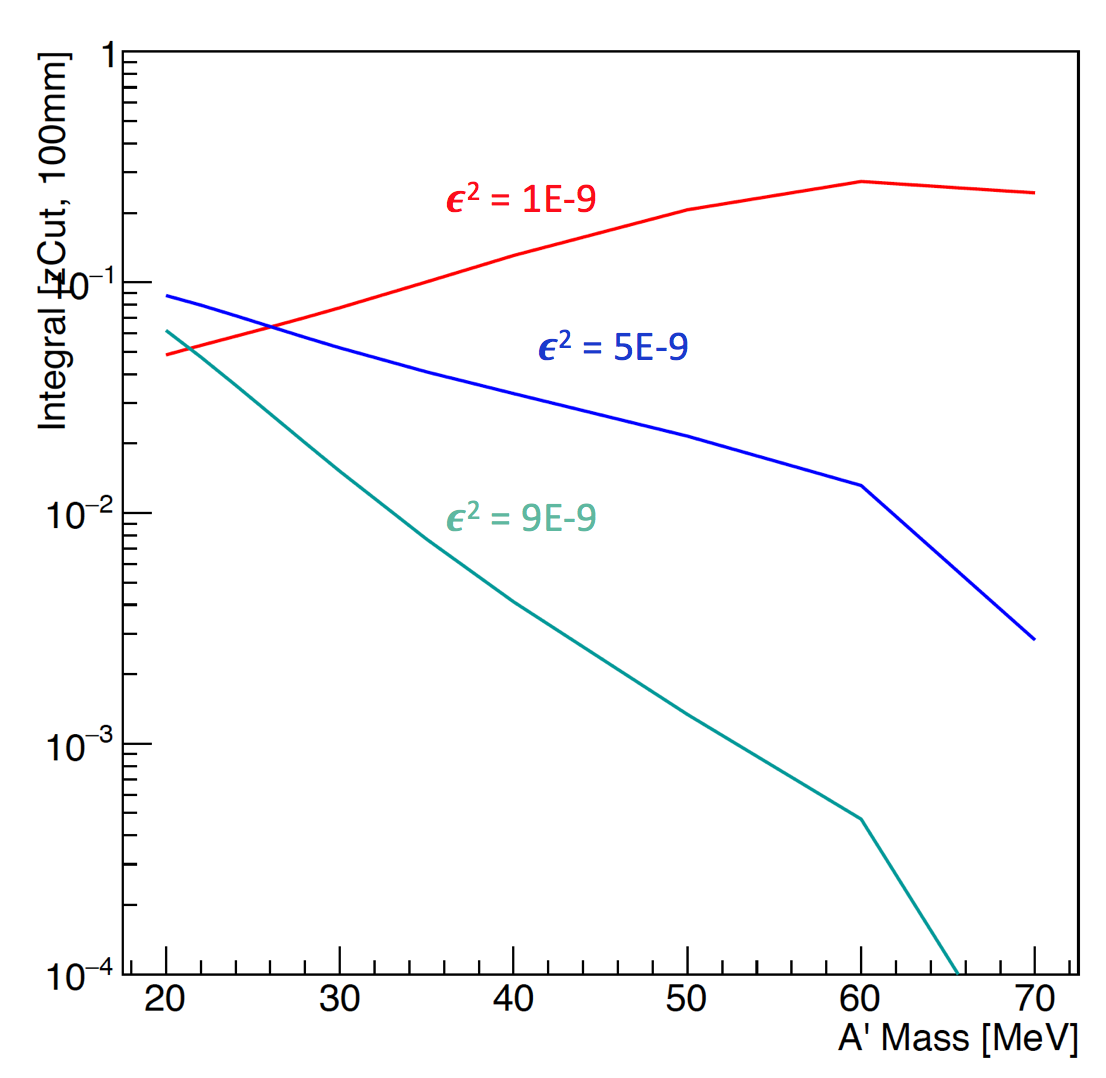
\includegraphics[width=0.8\textwidth]{plots/L1L1_eff1d.png}
  \caption{For a fixed $\epsilon^2$ coupling, the full integral value from zCut to the first layer of the SVT is shown as a function of mass. }
  \label{fig:integratedVal1D}
\end{figure} 

In the L1L1 dataset, the vertex reconstruction is most efficient for larger couplings as shown in Figure~\ref{fig:integratedVal1D}. Due to the geometric effects of the requirement to reconstruct tracks both passing through layer 1 of the SVT, the integral shows the highest efficiency for smaller couplings with larger masses.

\subsubsection{Mass resolution}

The mass resolution is determined from A' Monte Carlo and has been checked with the $e-e-$ mass resolution from Moller scattered electron pairs in data. By generating heavy photons at discrete masses, applying the cuts proposed in data, and fitting the A' mass peak residual with respect to the generated mass peak, the mass resolution can be measured as a function of mass. Fits to this peak are shown in Figure~\ref{fig:l1l1_mfits}.

\begin{figure}[H]
  \centering
     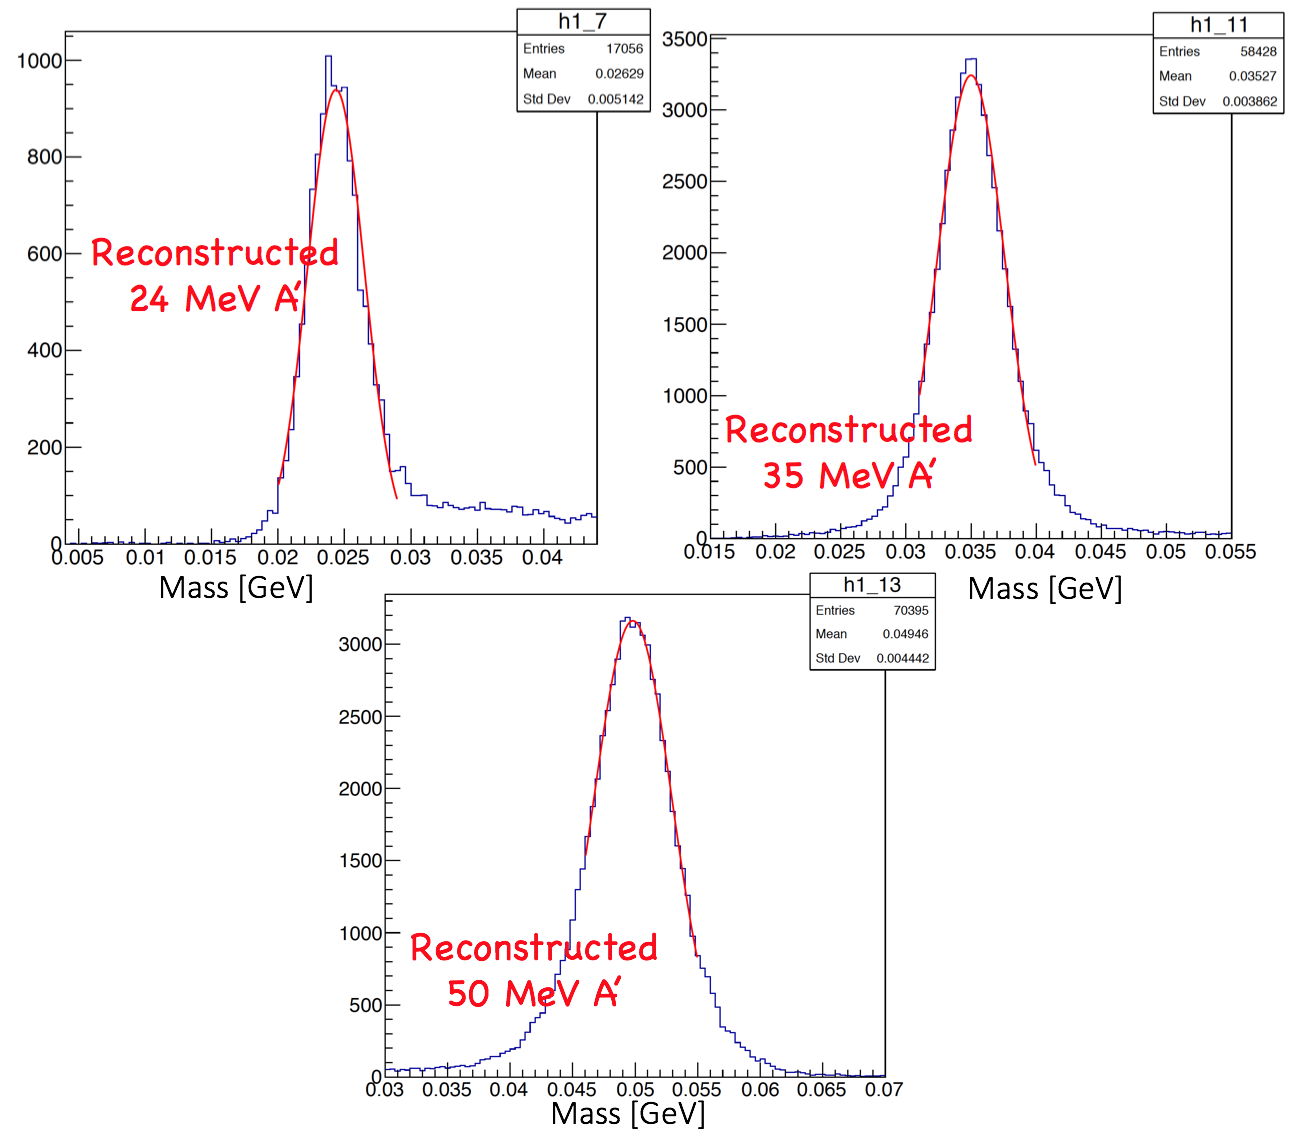
\includegraphics[width=0.8\textwidth]{plots/L1L1MassFit.png}
  \caption{Fits to the residual of the A' mass peak as reconstructed in Monte Carlo.}
  \label{fig:l1l1_mfits}
\end{figure} 

This resolution encompasses the measured angular resolution of the pair as well as the resolution of the measured momentum. It has been shown previously that while the mass resolution is dominated by the angular resolution term, there is no dependence with the vertex z position. The mass resolution as a function of mass using heavy photon Monte Carlo is shown in Figure~\ref{fig:massRes_L1L1}.


\begin{figure}[H]
  \centering
     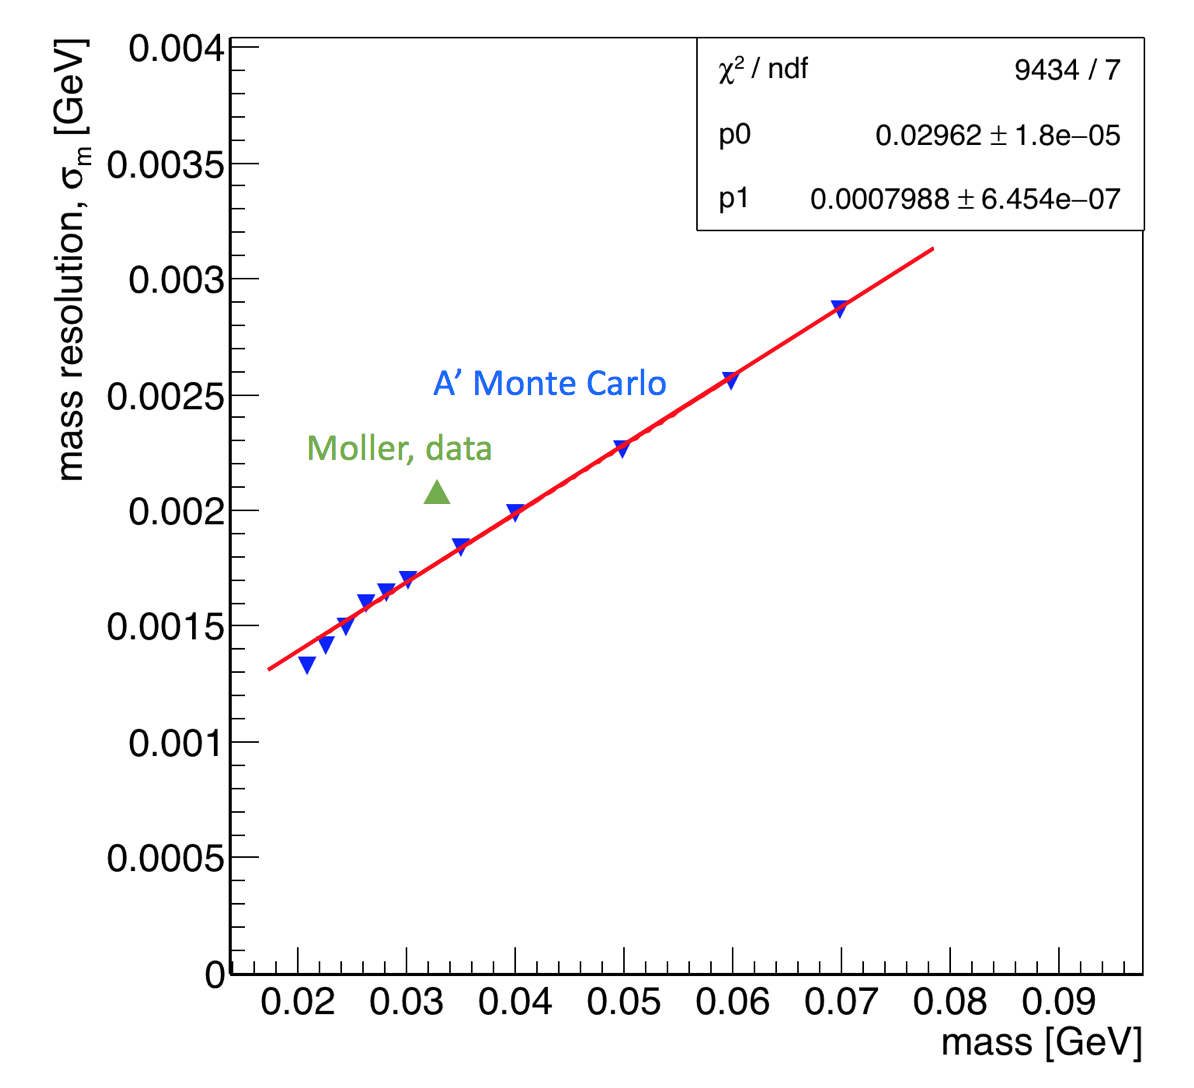
\includegraphics[width=0.8\textwidth]{plots/massRes_L1L1.png}
  \caption{The mass resolution from A' MC can be parameterized linearly as $p0m+p1$ with the fit values shown on the plot. The moller mass is one of the only real benchmarks to compare with the data and indicates a possible offset with the mass resolution measured in data. }
  \label{fig:massRes_L1L1}
\end{figure} 

Simulations of the Moller mass can be used to study systematic offsets between the measured mass in data and the mass as found in Monte Carlo. Using Moller Monte Carlo (with no beam background), the Moller mass can be seen in Figure~\ref{fig:mollerMC_L1L1}. 

\begin{figure}[H]
  \centering
     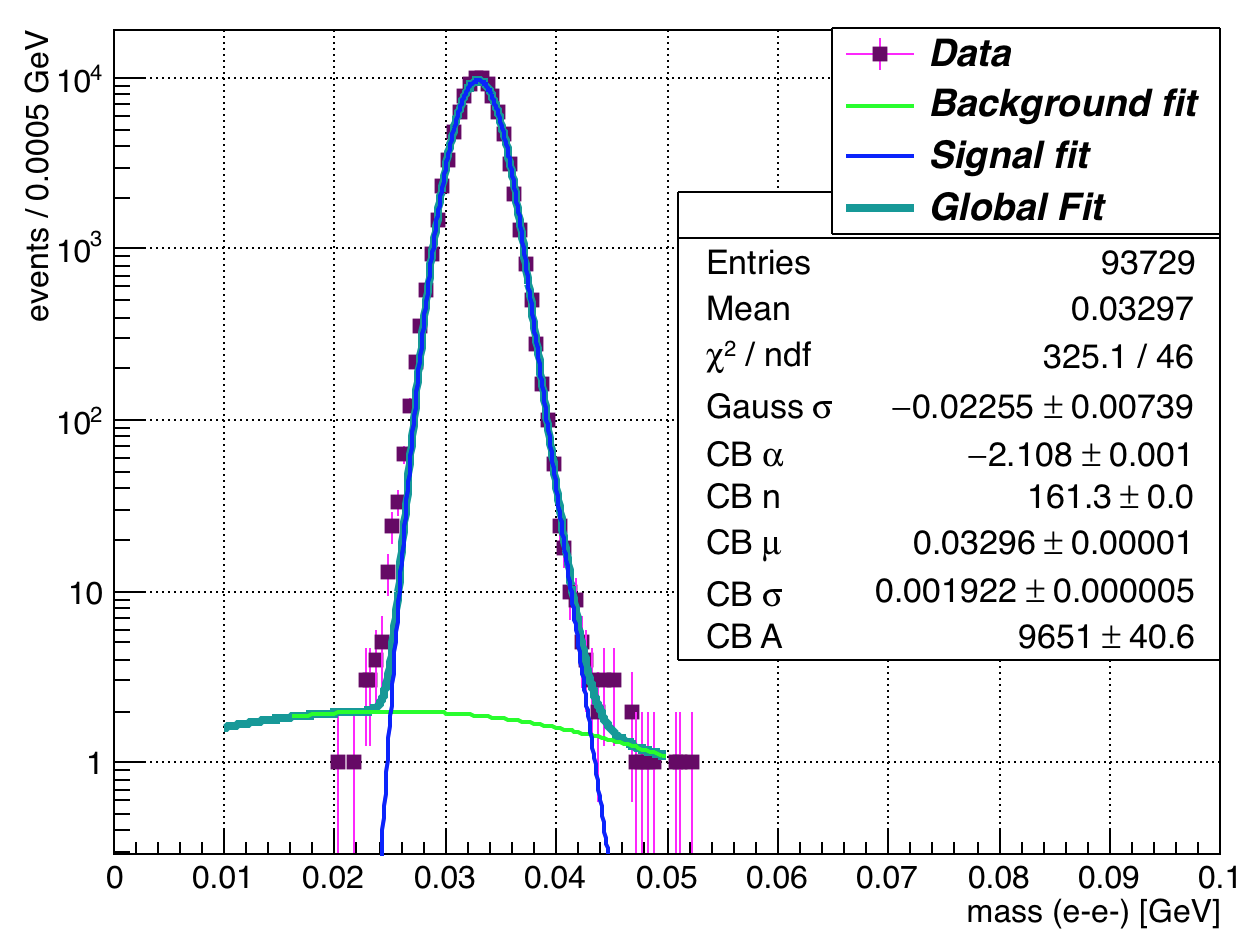
\includegraphics[width=0.8\textwidth]{plots/mollerMassMC.png}
  \caption{The fit to the moller mass peak as found in Monte Carlo is shown. The fit uses a crystal ball function to describe the signal and a Gaussian to fit the low background under the peak.}
  \label{fig:mollerMC_L1L1}
\end{figure}

The Moller mass from Monte Carlo can be immediately compared with the Moller mass as found in data. The difference in resolution between the peak from the pure Monte Carlo Moller sample and the Moller sample in data is approximately 17$\%$. This difference should be applied to the heavy photon mass resolution found in Monte Carlo in order to appropriately scale the bin widths when slicing and fitting the vertex distribution by mass. The Moller peak from data is shown in Figure~\ref{fig:moller_L1L1}. 

\begin{figure}[H]
  \centering
     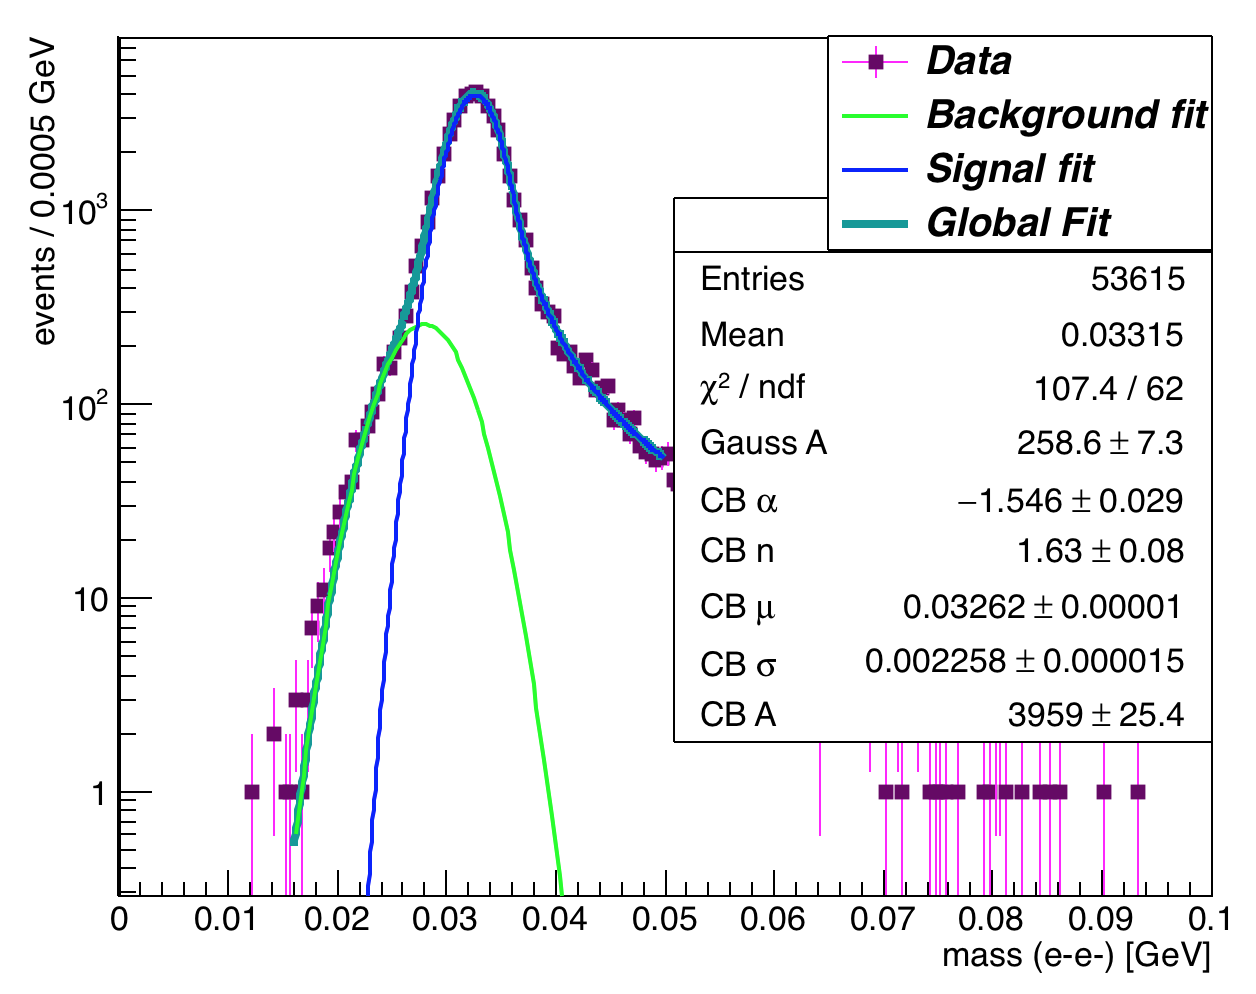
\includegraphics[width=0.8\textwidth]{plots/mollerMass.png}
  \caption{The fit to the Moller mass peak as found in data is shown. The fit uses a crystal ball function to describe the signal and a Gaussian to fit the low mass background side to the peak.}
  \label{fig:moller_L1L1}
\end{figure} 

After applying the 17$\%$ scaling to the mass resolution from A' Monte Carlo, we obtain the mass resolution in Equation~\eqref{eq:massresSl1l1}.

\begin{equation}
\label{eq:massresSl1l1}
\sigma_m = 0.02428m+0.000787
\end{equation}

The scaled mass resolution in Equation~\eqref{eq:massresSl1l1} is used in the vertex analysis to find the $z$ vertex cut. 

 \subsubsection{Accidentals}

The effects of accidentals on the vertex backgrounds must be understood if one is to understand the signal significance after unblinding. The rigorous way to accomplish this can be done by selecting electrons and positrons from different beam buckets and vertexing these pairs to create a high statistics sample to study. As the ability to vertex pairs from different beam buckets is not yet implemented in the HPS software, we can select $e+e-$ pairs with larger than 3~ns time difference and less than 9~ns time difference. As we go to larger time differences, we begin to lose events due to the SVT inefficiency outside of the trigger window. The final data selection cut is for clusters that are within $\pm$2~ns and includes two beam buckets. By looking for high z vertices generated in the six out of time beam buckets, we can obtain an estimate for the number of accidentals we will expect to see when we unblind. For the L1L1 dataset, the vertex distribution for the selected accidentals is shown in Figure~\ref{fig:acc_L1L1}.

\begin{figure}[H]
  \centering
     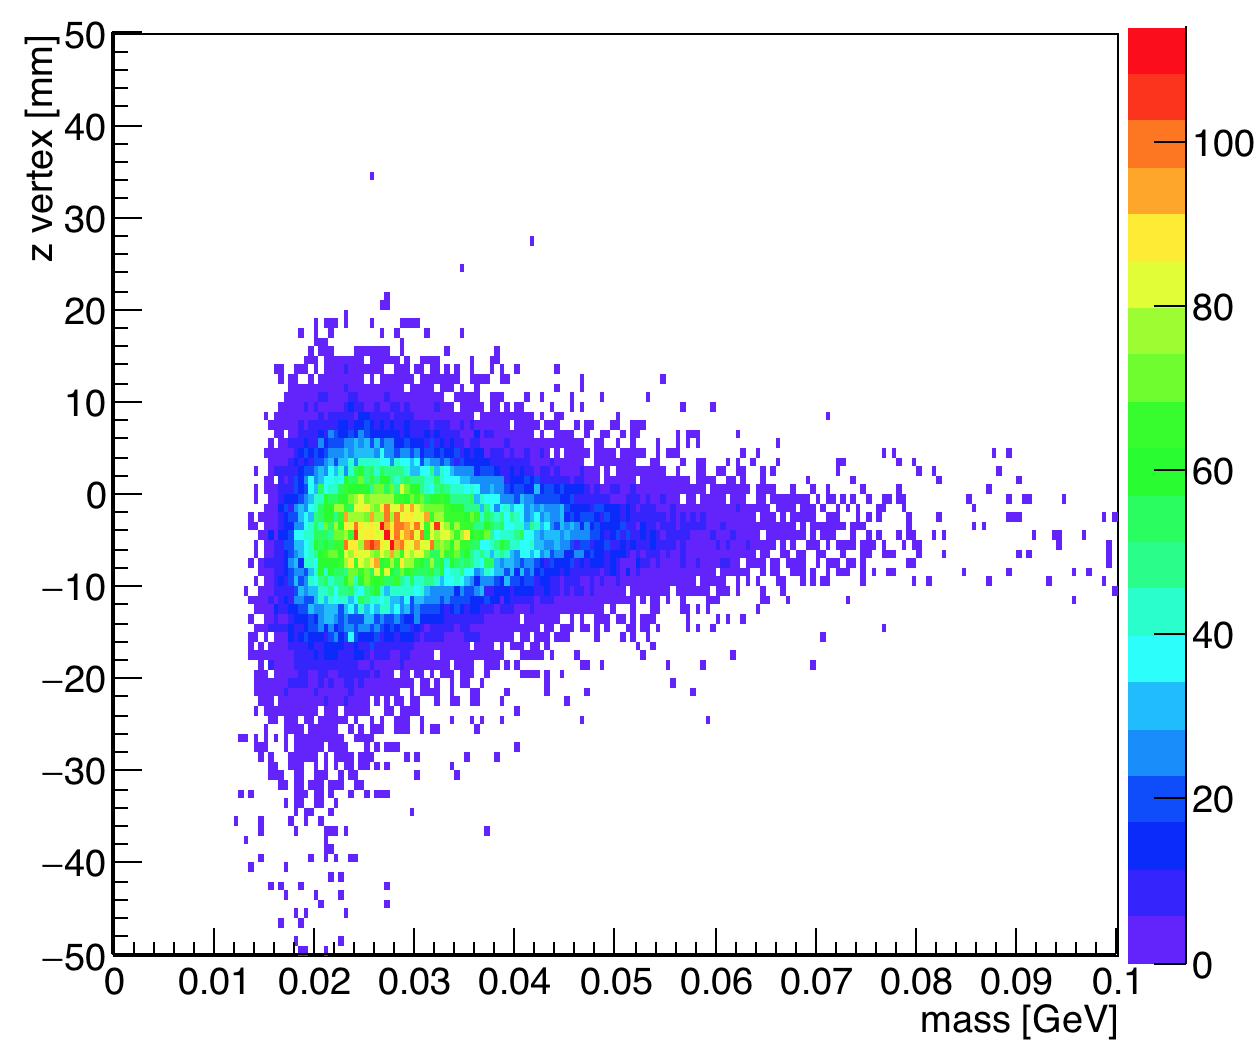
\includegraphics[width=0.8\textwidth]{plots/zVm_acc_L1L1.png}
  \caption{After selecting events where the cluster time difference is greater and 3~ns and less than 9~ns, the vertex distribution for the six beam buckets is shown.}
  \label{fig:acc_L1L1}
\end{figure} 

As seen in Figure~\ref{fig:acc_L1L1}, there are 3 visible high z events. If we translate this effect to the two beam buckets in our selected events peak, we could expect $1\pm0.6$ accidental events in the 10$\%$ unblinded data. This could account for $10\pm6$ events in the full 100$\%$ dataset. It is worth noting that the high z background events appear to be randomly distributed among the mass bins.

\subsubsection{Projected reach}

We estimate our reach by using Equation~\eqref{eq:signal}. In order to establish 90$\%$ confidence limits, we should expect to see 2.3 events or greater in the corresponding mass bin. The resultant z vertex distribution as a function of mass for the L1L1 dataset is shown in Figure~\ref{fig:zVm_L1L1}.

\begin{figure}[H]
  \centering
     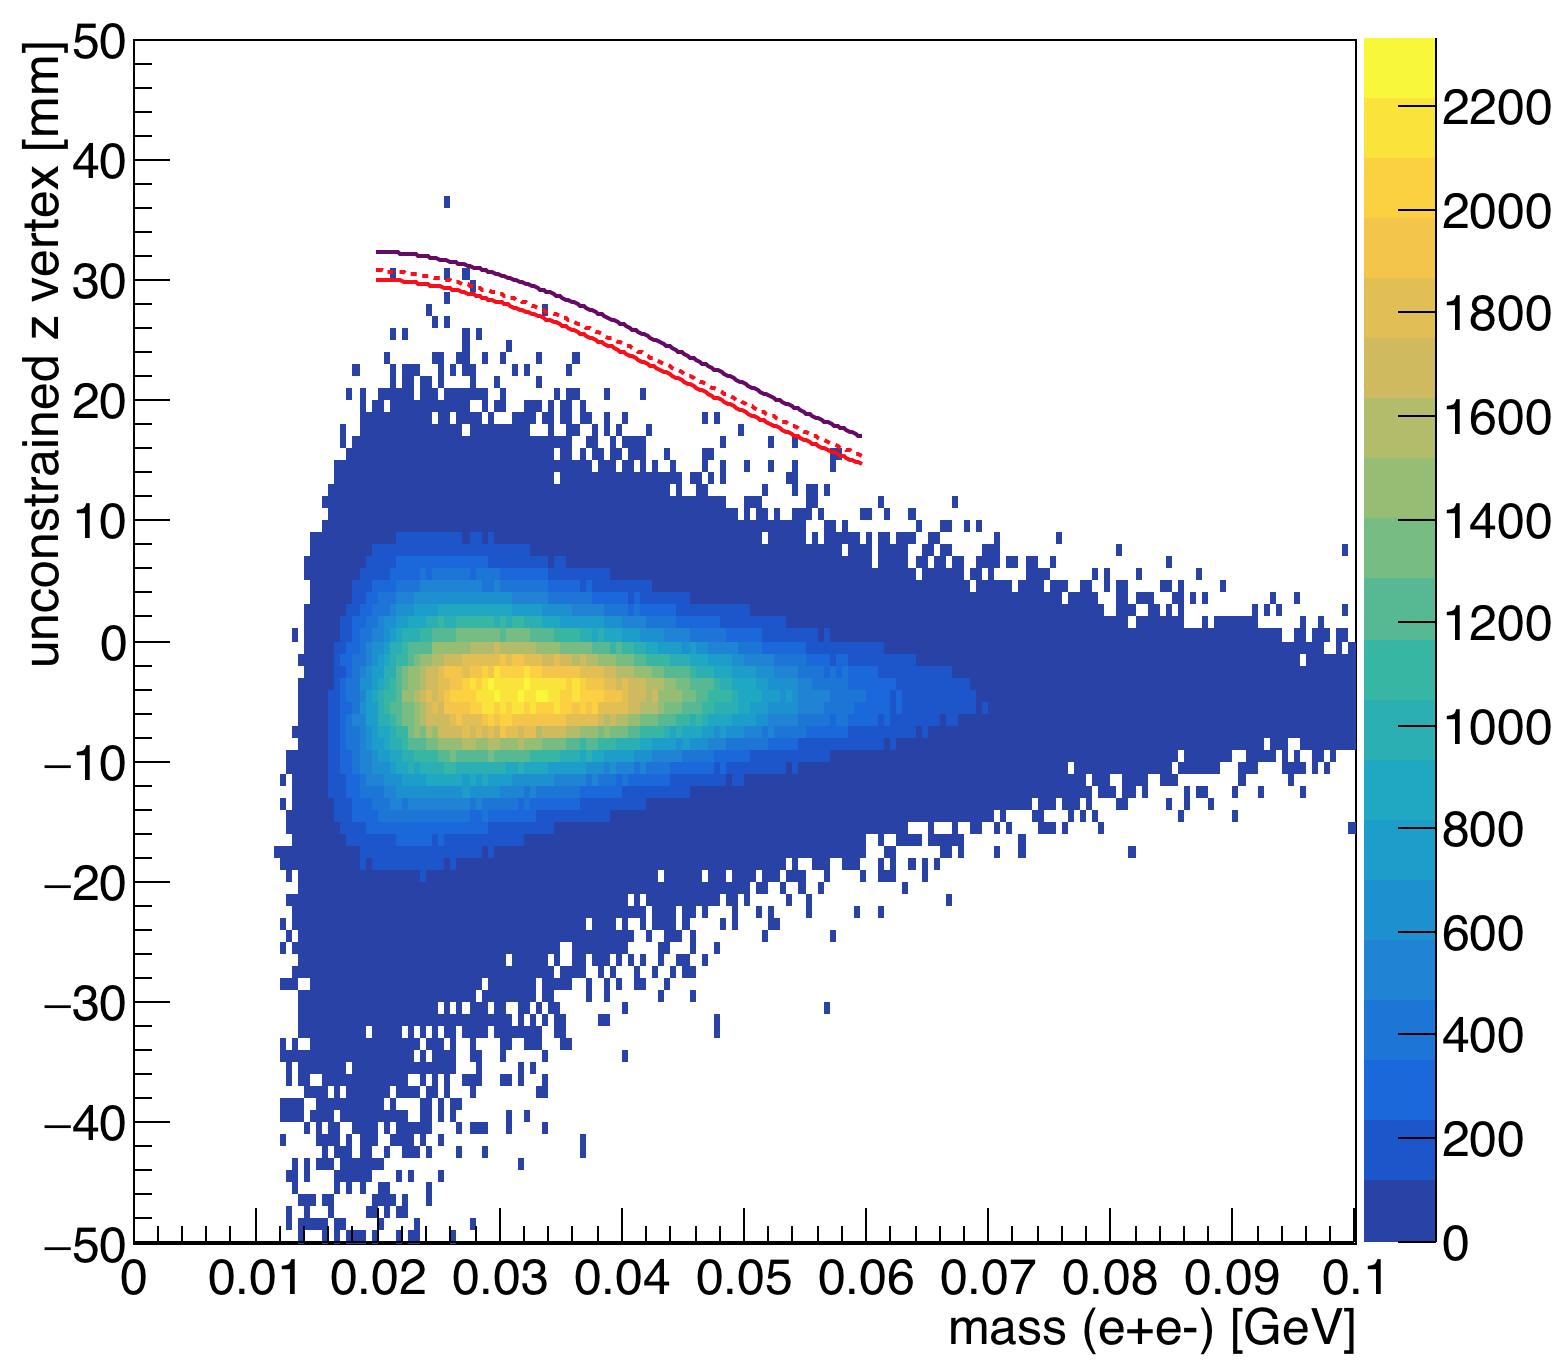
\includegraphics[width=0.8\textwidth]{plots/zVm_L1L1_0p5.png}
  \caption{Reconstructed z vertex as a function of mass for the L1L1 dataset with the first layer of the SVT at 0.5~mm from the beam. The solid red line indicates the zCut found for 10$\%$ of the data (unblinded), and the dashed red line indicates the limit at which events have a quantile greater than 0.5 with respect to the predicted background model. The purple line shows where the projected zCut will be for the full dataset after unblinding.}
  \label{fig:zVm_L1L1}
\end{figure}

As shown in Figure~\ref{fig:zVm_L1L1}, we see the zCut found for the 10$\%$ data sample after fitting the peaks and looking for the location where we have 0.5 background events in the bin. Because we have an average of 0.5~background events in each bin, we characterize the events that lie beyond the zCut using the distribution function of the exponential model for the tail. A quantity between 0 and 1 can tell us how far an event located at a particular z value, relative to the zCut, is from being described by the background function. This distribution is described in terms of the tail length, $l$, by $1-e^{(zCut - z)/l}$ and can be inverted to find the value of z relative to the zCut yielding a specific quantile. All but one event that lie beyond the zCut can be explained in accordance with the background model. After unblinding, high z events will be further investigated, and it's possibly attributable to the estimate on the rate of accidental contamination in the sample.\\

The final reach with the projected zCut for the 100$\%$ L1L1 dataset is shown in Figure~\ref{fig:zVm_reach}.

\begin{figure}[H]
  \centering
     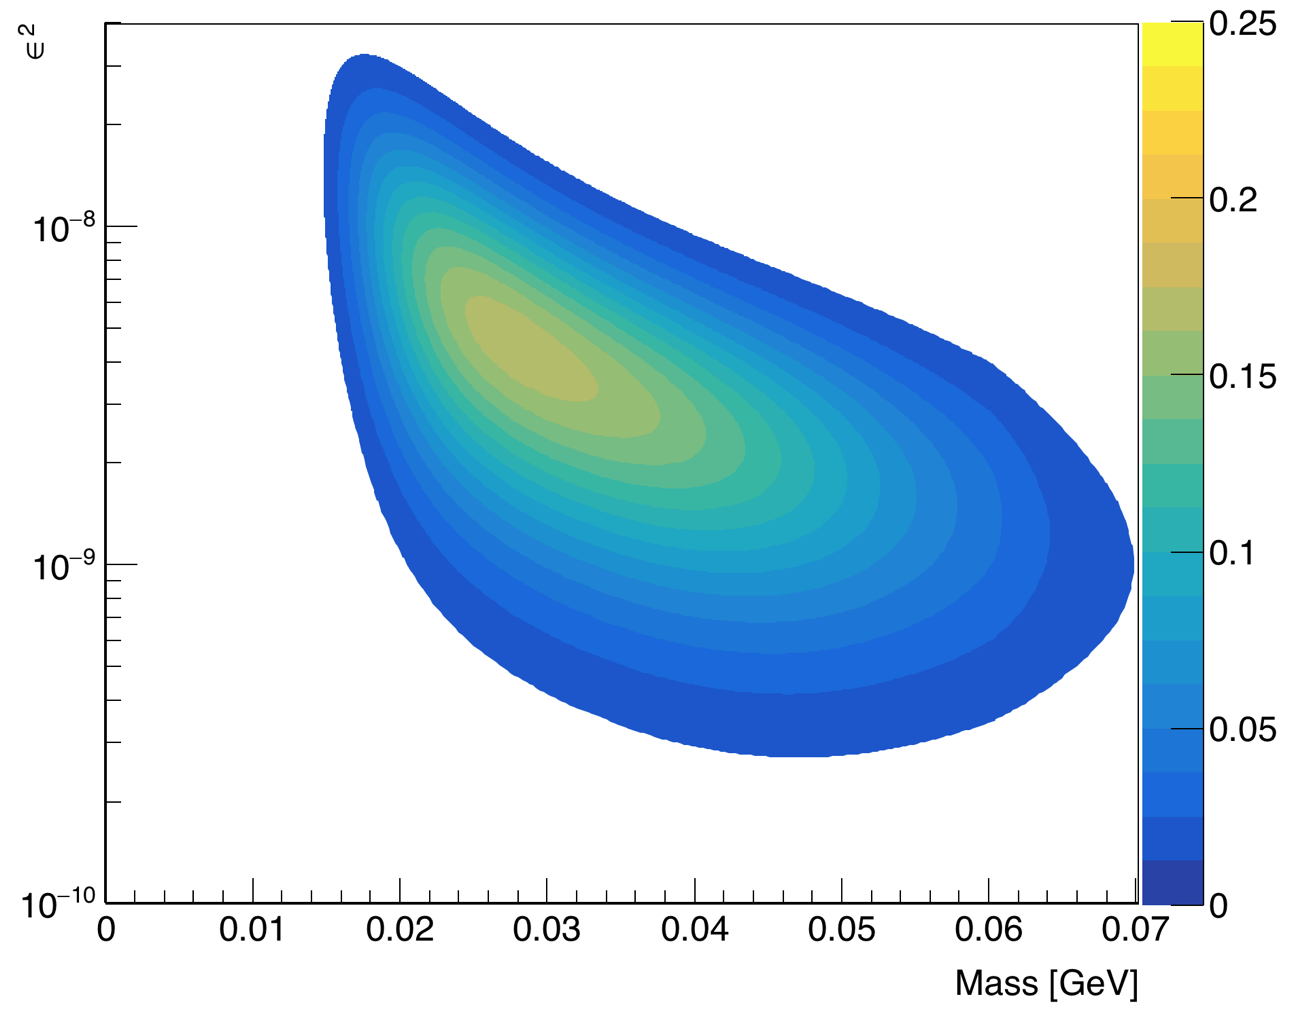
\includegraphics[width=0.8\textwidth]{plots/reachL1L1.png}
  \caption{The expected signal yield for the full 0.5~mm 100$\%$ dataset. This uses the zCut projection shown in Figure~\ref{fig:zVm_L1L1}.}
  \label{fig:zVm_reach}
\end{figure} 

As seen in Figure~\ref{fig:zVm_reach}, the highest signal count that can be expected from the full dataset is 0.21 events. This reach is only for the L1L1 dataset and only accounts for 1.7~days of beam time. 
